\begin{savequote}[100mm] 
Machines take me by surprise with great frequency.
\qauthor{Alan Turing} 
\end{savequote}

\chapter{A reconfigurable two-qubit chip}
\label{chap:cnot-mz}

\section{Introduction}
\label{sec:cnot-mz-intro}
The discovery and development of universal computing machines is one of the greatest scientific accomplishments of the 20$^{\text{th}}$ century. The Church-Turing thesis --- that all calculable functions can be computed by a particularly simple type of machine --- is generally expressed as a statement about mathematical functions, and the evaluation of numbers. However, the influence of universal computing machines has stretched much further than the academic mathematical context in which they were first conceived, having profound effects on social, economic and artistic life.

The prospective benefits of quantum computing enjoy a similar promise of universality. Specifically, we believe \cite{Deutsch1985} that a scalable machine satisfying the DiVincenzo criteria (section \ref{sec:divincenzo-criteria}) would be universal for quantum computing, and could run any quantum algorithm, prepare any quantum state or operator\footnote{Note that this does not imply any particular scaling: arbitrary $N$-qubit state preparation is exponentially hard even for quantum computers. See chapter \ref{chap:quantum-chemistry} for further discussion.}, and would also be universal for classical computation. This promise allows us to progress with the development of the basic building blocks of quantum information technologies, without complete information on the potential applications of quantum computing: although we have a small number of specific examples of quantum algorithms which provide an exponential speedup over classical machines, it is reasonable to think that, as with classical computation, the scope of useful applications will ultimately prove to be much broader.

The results of \acrshort{klm} (section \ref{sec:klm}), together with more recent developments in cluster-state theories \cite{Raussendorf2001, Raussendorf2003, Briegel2001, Browne2005}, show that in principle \acrshort{loqc} can provide a scalable route to universal quantum computation. More recently, integrated quantum photonics (section \ref{sec:integrated-quantum-photonics}) has been shown to offer an \emph{experimentally} scalable approach to the construction of \acrshort{loqc} machines, potentially allowing millions  \cite{Sun2013} of components to be lithographically fabricated on a single monolithic chip. Early results in the field include the demonstration of quantum interference in passive linear optical interferometers \cite{Politi2009, Laing2010, Marshall2009, Peruzzo2011a}, as well as active devices with reconfigurable phase shifters\cite{Matthews2009, Matthews2011a, Bonneau2012b}. Notably, most of these reconfigurable devices used a single phase shifter, giving the device a single classical control parameter. This was sufficient for novel demonstrations of quantum metrology \cite{Matthews2009} and switching of entangled photonic states \cite{Bonneau2012b}. However, much of the utility and interest of a universal quantum computer arises from the fact that a single machine can be arbitrarily reconfigured to perform a broad variety of tasks. This degree of reconfigurability requires a large (polynomial) number of classical control parameters, and is the main focus of work described in this section.

We describe a waveguide linear-optical circuit which can encode and manipulate the state of two photonic qubits using two indistinguishable photons from an \acrshort{spdc} source. This device features eight voltage-controlled phase shifters, which can be arbitrarily reconfigured to prepare any two-qubit state. The architecture of the device includes four reconfigurable single-qubit operations, together with a passive two-qubit entangling gate. As such, the gate operations implemented in this device comprise a universal quantum gate set (section \ref{sec:divincenzo-criteria}). 

In close analogy with classical computers, we find that the degree of reconfigurability afforded by this device has allowed a surprisingly rich variety of physical phenomena and quantum information techniques to be studied, above and beyond the original intent of the device. Indeed, chapters \ref{chap:delayed-choice}, \ref{chap:random-chsh}, and \ref{chap:quantum-chemistry} all make use of the two-qubit chip described here. This work highlights the fact that nontrivial experiments can be performed using even a very small number of qubits, in contrast with the classical case --- where the scope of worthwhile experiments using only two classical bits is limited.

To our knowledge, this work includes the first experimental implementation of photonic two-qubit quantum state and process tomography (where state preparation and measurement were performed on-chip), and the first photonic on-chip Bell inequality violation.

\section{\acrshort{cnotmz}}

% %%%%%%%%%%%%%%% CNOT-MZ main figure
\begin{figure}[t!]
\centering
\includegraphics[width=\linewidth]{chapter3/fig/newchip.pdf}
\caption[\acrshort{cnotmz} chip]
{\acrshort{cnotmz} chip. (a) Circuit-model diagram. Two qubits are prepared in the \ket{00} state. $H'$ is a Hadamard-like gate corresponding to a directional coupler, with the same unitary matrix representation as a beamsplitter (\ref{eqn:beamsplitter-unitary}). $R_z(\phi)$ correspond to voltage-controlled phase shifts, and implement single-qubit rotations about the $z$-axis of the Bloch sphere (\ref{eqn:phase-shift-unitary}). At the centre of the chip is a two-qubit \acrshort{cnotp} entangling gate, locally equivalent to the maximally entangling \acrshort{cnot} gate. Each qubit can be effectively measured in an arbitrary basis, by combining single-photon rotations with measurement in the $z$-basis. (b) Waveguide architecture. All \glspl{dc} have coupling ratio $\eta=1/2$, apart from $c_6$ ,$c_7$ and $c_8$, which are engineered to transmit a fraction $\eta=t=2/3$ of incident light. 
Two indistinguishable photons generated by type-I \gls{spdc} are coupled into the chip, and encode two qubits in path. Waveguides $w_{2,3}$ and $w_{4,5}$ correspond to the $\ket{0}$ and $\ket{1}$ states of the control and target qubit respectively. Waveguides $w_1$ and $w_6$ do not correspond to logical basis states. The first stage of the chip uses two \glspl{mzi} and four phaseshifters to implement arbitrary two-qubit separable state preparation. The central section implements the \acrshort{cnotp} gate. The final section of the chip uses two \glspl{mzi}, together with off-chip single-photon detection, to implement arbitrary separable two-qubit measurements. }
\label{fig:cnot-mz-chip}
\end{figure}
% %%%%%%%%%%%%%%% End CNOT-MZ main figure

The \acrshort{cnotmz} is a reconfigurable quantum photonic chip, shown schematically in figure \ref{fig:cnot-mz-chip}(b). Two qubits are encoded in path, using indistinguishable photon pairs at \SI{808}{\nano \metre}, generated by type-I \acrshort{spdc}. The chip uses a total of 6 waveguides, 13 directional couplers and 8 voltage-controlled thermal phaseshifters to implement the circuit model diagram shown in figure \ref{fig:cnot-mz-chip}(a). 

The architecture of the chip is based around a passive \gls{cnotp} gate, which implements a maximally entangling \gls{cnot}-like operation on the two qubits. This gate is discussed in detail in section \ref{sec:ralph-cnot}. The control qubit is encoded using waveguides $w_2$ and $w_3$, corresponding to the $\ket{0}$ and $\ket{1}$ states respectively, and the target qubit is similarly encoded across $w_4$ and $w_5$. Each qubit is initially prepared in the $\ket{0}$ state, with photon pairs coupled directly from the source into waveguides $w_2$ and $w_4$. Arbitrary state preparation of each qubit is then accomplished using an MZI with two phaseshifters, as described in section \ref{sec:cnotmz-state-preparation}. At the output of the \gls{cnotp} gate, each qubit is measured in a local basis using an MZI together with two single-photon detectors, as described in section \ref{sec:cnotmz-measurement}.

The device was fabricated by CIP technologies \cite{CIP} in a silica-based material system, described in section \ref{sec:silica-on-silicon}. The chip die is \SI{3}{\milli \metre} wide and \SI{70}{\milli \metre} long. Full details of the photon source, control system and supporting experimental setup are given in section \ref{sec:cnotmz-experimental-setup}.

\subsection{Silica-on-Silicon} 
\label{sec:silica-on-silicon}
% %%%%%%%%%%%%%%% Silica on silicon figure
\begin{figure}[t!]
\centering
\includegraphics[width=\linewidth]{chapter3/fig/silica_on_silicon.pdf}
\caption[Silica on silicon]
{Silica-on-silicon material system and waveguide geometry. Square \SI{2.5}{\micro\metre} $\times$ \SI{2.5}{\micro\metre} waveguides were fabricated in germanium/boron-doped silica, on a silicon substrate. The waveguide cladding is a combination of undoped silica and phosphorous/boron-doped silica. Titanium/platinum/gold traces connect to titanium/platinum resistive heaters, allowing a reconfigurable voltage-controlled phase shift to be applied. Contact pads were gold-wire-bonded to a standard \gls{pcb}.}
\label{fig:silica-on-silicon}
\end{figure}
% %%%%%%%%%%%%%%% End silica-on-silicon figure

Glass (silica) waveguides are particularly well-suited for quantum applications. 
In particular, they exhibit very low propagation loss (\SI{<0.1}{\dB \per \centi \metre}), couple well to single-mode optical fibre (typically \SI{\sim 70}{\percent} coupling efficiency), and are transparent to the band around \SI{\sim 800}{\nano \metre} where \gls{spdc} sources and room-temperature \gls{apd} single-photon detectors are most efficient.  Propagation/coupling loss and detection efficiency are particularly important in multiphoton experiments, where the $N$-photon detection rate typically falls off exponentially with overall loss $\eta$ as $1/\eta^N$. The main disadvantage of this material system is the limited refractive index contrast, typically on the order of $\Delta=0.5\%$. This imposes a large minimum waveguide bend radius of \SI{\sim 15}{\milli \metre} (see section \ref{sec:guided-modes}), leading to \SI{200}{\micro\metre}-wide directional couplers on the order of \SI{\sim 6}{\milli \metre} in length. Recently, more compact devices have been achieved using alternative material systems, at the cost of greater loss (see sections \ref{sec:quantum-walk-chip}, \ref{sec:bosonsampling-chip} and \ref{sec:cnotmz-discussion}).

The \acrshort{cnotmz} device was fabricated using silica-on-silicon planar lightwave circuit technology, shown in figure \ref{fig:silica-on-silicon}.  
A \SI{16}{\micro \metre} buffer layer of undoped silica was grown on a silicon substrate, forming the lower cladding of the waveguides. A \SI{3.5}{\micro \metre} layer of silica doped with germanium and boron oxides was overgrown, and was then lithographically etched to form the square \SI{3.5}{\micro \metre} $\times$ \SI{3.5}{\micro \metre} waveguide core, with a refractive index contrast between core and cladding of $\Delta=0.5\%$. A \SI{16}{\micro \metre}-thick upper cladding of silica, doped with phosphorous and boron to match the lower cladding, was then overgrown. Finally, a metallic layer was deposited and lithographically etched to form resistive heaters, electrical connections, and probe contact pads on the top surface of the chip. 

The waveguides used here have a symmetric (square) profile, which together with the amorphous, isotropic nature of silica leads to negligible birefringence. As a result, in principle these waveguides will support any single polarization of light. Although on-chip polarization encoding has been demonstrated in a number of material systems \cite{Bonneau2012b, Dai2012, Crespi2011}, it remains challenging --- in particular due to unwanted rotations introduced by waveguide bends --- and in this work we operate in vertical polarization only.

\subsection{Directional Coupler} 
\label{sec:directional-coupler}
% %%%%%%%%%%%%%%% Directional coupler figure
\begin{figure}[t!]
\centering
\includegraphics[width=.7\linewidth]{chapter3/fig/directional_coupler.pdf}
\caption[Directional coupler]
{Geometry of a directional coupler. Two waveguides are adiabatically brought into close proximity, such that the evanescent fields overlap. Light periodically couples from one waveguide to the other as a function of the propagation distance $L$ and the coupling constant $\kappa$, which depends in part on the spatial separation $s$ and refractive index $n$.}
\label{fig:directional-coupler}
\end{figure}
% %%%%%%%%%%%%%%% End Directional coupler figure
Leading approaches to the implementation of two-mode beamsplitter operations in integrated photonics include \gls{mmi} couplers and \glspl{dc}. Here we consider the latter, illustrated in figure \ref{fig:directional-coupler}, in which two waveguides are brought close together so as to couple the guided modes via the evanescent field (section \ref{sec:guided-modes}). Any \gls{dc} is characterised by its coupling ratio $\eta$, corresponding to the fraction of optical power transmitted from one waveguide to the other, which is equivalent to the \gls{bs} transmissivity (section \ref{sec:beamsplitter}) and is controlled by the separation distance $s$ and length $L$ of the coupling region.

%Quick description of coupling
\emph{Mode coupling theory} \cite{Lifante2003} gives the relationship between the field amplitude (\ref{eqn:infinite-field}) in two coupled waveguides $A$, $B$ as a system of coupled differential equations
\begin{equation}
   \frac{dA(z)}{dz}  = - i \kappa B(z) ~; \quad 
   \frac{dB(z)}{dz}  = - i \kappa A(z),
\end{equation}
where $\kappa$ is a coupling constant which depends on the spatial overlap of the two guided modes. This leads to solutions of the form
\begin{equation}
    A(z) = A_0 \cos(\kappa z) - B_0 i \sin(\kappa z)~;\quad
    B(z) = B_0 \cos(\kappa z) - A_0 i \sin(\kappa z),
\end{equation}
where $A_0$, $B_0$ are the initial field amplitudes at the input ports. As a result, in the coupling region of the \gls{dc}, optical power oscillates sinusoidally between the two waveguides as a function of the interaction length $L$. By tuning this length, the \gls{dc} can be designed to implement an arbitrary \gls{bs} operation (\ref{eqn:beamsplitter-unitary})
\begin{equation}
\begin{bmatrix} A(L)\\ B(L)\end{bmatrix} 
=
\begin{bmatrix} 
 \cos(\kappa L)  & -i \sin (\kappa L)\\
-i \sin(\kappa L) & \cos (\kappa L)
\end{bmatrix} 
\begin{bmatrix} A_0\\ B_0\end{bmatrix} 
=
\transfer_\text{DC} (\kappa, L) 
\begin{bmatrix} A_0\\ B_0\end{bmatrix} 
=
\begin{bmatrix} 
\sqrt{t}  & i \sqrt{r}\\
i \sqrt{r}  & \sqrt{t}
\end{bmatrix} .
\end{equation}
In order to obtain a 50:50 \gls{dc} with $t=r=\frac{1}{2}$, we must therefore have $L=\pi/4 \kappa$, which for the silica-on-silicon material system used here, with $s=\SI{3}{\micro\metre}$, corresponds to an interaction length of \SI{\sim 4}{\milli \metre}.

%How well it can be fabricated
The quality of fabrication of directional couplers is critical to the performance of the \gls{cnotmz} and other linear-optical quantum circuits described in this thesis. Deviation from the designed coupling ratio leads to unitary errors in qubit state preparation and measurement, and reduces the contrast of classical interference. Moreover, errors in both coupling ratio and imperfect mode-matching at the interaction region of the coupler lead to reduced visibility of \gls{hom} interference, and thus contribute to the observed sub-unit quantum state/process fidelities reported in sections \ref{sec:state-tomography}, \ref{sec:cnot-process-tomography} of this thesis.

\subsection{Thermal Phaseshifter} 
\label{sec:thermal-phaseshifter}
%Motivate
The general-purpose flexibility of the \gls{cnotmz} is achieved through the inclusion of eight reconfigurable phase shifters, as shown in figure \ref{fig:cnot-mz-chip}. 
In silica-on-silicon, reconfigurable phase shifts are most easily implemented using the \emph{thermo-optic effect}. Here, a metallic (titanium/platinum) resistive heater of length $L$ is lithographically patterned on the top surface of the upper waveguide cladding, directly above the waveguide core, as shown in figure \ref{fig:silica-on-silicon}. This heater is connected via Ti/Pt/Au electrodes to a current source, allowing the temperature of a local region of the waveguide to be precisely controlled via Ohmic heating. This gives rise to a to a change in the refractive index of the local core and cladding, with $dn/dT \sim 10^{-5} / \text{K}$, increasing the effective path length and leading to a phase shift $\varphi$ with respect to the unperturbed waveguide. 

The maximum temperature difference supported by the silica-on-silicon material system is \SI{\sim 30}{\degree}C, and in order to achieve a range in phase of 2$\pi$ the resistive heater must therefore have a length on the order of \SI{4}{\milli \metre}. 
The heaters are rated for a maximum voltage of \SI{5}{\volt}, however in order to achieve a full $2\pi$ phaseshift in all \glspl{mzi} we had to exceed this limit, running most phaseshifters between \SI{0}{\volt} and \SI{7}{\volt}, leading to a total of  \SI{\sim 1}{\watt} per heater at maximum voltage. I-V curves for each resistive heater on the \gls{cnotmz} are shown in figure \ref{fig:calibration}(d), showing a typical resistance of $R$ \SI{\sim 60}{\ohm}. Further details of phaseshifter calibration are given in section \ref{sec:cnot-mz-calibration}.

%Drawbacks
The main drawback of thermal phase shifting is switching speed: in the silica-on-silicon platform used here, heating/cooling of a phaseshifter for a differential phaseshift of $\pi$ takes at least \SI{\sim 100}{\milli \second} (figure \ref{fig:calibration}(c, inset)). This limits the scope of applications --- for instance, active feed-forward is not possible using this technology. However, in the majority of experiments described in this thesis, the time taken to acquire a sufficient number of single-photon detection events, corresponding to a single measurement of an expectation value, is typically at least \SI{1}{\second}, and in practice there was not any need to switch phases faster than \SI{1}{\hertz}. Alternative material systems for integrated quantum photonics support an electro-optic effect, where phase can switched electrically up to \si{\giga \hertz} frequencies. See \cite{Bonneau2012b} for an example in lithium niobate.

\subsection{Linear-optical \acrshort{cnotp} gate} 
\label{sec:ralph-cnot}
%\gls{klm} (\ref{sec:klm}) have shown that universal quantum computation can be achieved using linear optics together with single-photon sources, single-photon detectors, and active feed-forward. 
It was shown by Lloyd \cite{Lloyd1995a} that almost any two-qubit entangling gate is universal for quantum computing, and by DiVincenzo that a universal gate set can always be constructed from a two-qubit entangling gate together with single-qubit rotations \cite{DiVincenzo1995}.
We have seen in section \ref{sec:mach-zehnder-interferometer} that deterministic, arbitrary single-qubit rotations are very easily constructed using linear optics.
However, since photons do not interact, the greatest challenge (and the greatest accomplishment of \gls{klm}), is to find a scalable two-qubit entangling gate.  All scalable approaches to \gls{loqc}, including \gls{klm} and more recent cluster-state techniques (section \ref{sec:klm}, \ref{sec:errors-in-quantum-computers}), depend on active feed-forward. At the time of writing, although fast switching, low propagation loss, high refractive-index contrast, integrated \si{\giga \hertz} logic and single-photon detectors, etc. have all been demonstrated in separate photonic devices, no existing technology or material system satisfies all necessary conditions for a full demonstration of scalable \gls{loqc} with active feed-forward. Certainly, the thermal phase-shifters previously described are too slow for such applications.

In 2002, two groups \cite{Ralph2002, Hofmann2002} proposed a scheme by which a two-qubit maximally-entangling gate can be implemented using linear-optics and postselection, without any need for feed-forward. It has already been stated (section \ref{sec:klm}) that \gls{loqc} is not scalable without feed-forward, and indeed this gate does not scale --- successful operation of the gate is postselected with probability $1/9$, leading to exponentially decreasing success probability for composite circuits. However, the scheme is experimentally much more accessible, and an experimental demonstration was almost immediately reported  by a number of groups \cite{Franson2002, Pittman2002, OBrien2003, Gasparoni2004}.
An important property of the design of this postselected gate is that it possesses many of the same experimental prerequisites --- indistinguishable photons, high visibility classical and quantum interference, stable interferometers --- as the scalable \gls{cz} gate of \gls{klm}, and experimental implementations of the former thus constitute real progress towards the latter.

% %%%%%%%%%%%%%%% CNOT-P gate
\begin{figure}[t!]
\centering
\includegraphics[width=0.9\linewidth]{chapter3/fig/cnotp.pdf}
\caption[\acrshort{cnotp} gate construction]
{
\gls{cnotp} gate construction. (a) Postselected linear-optical \gls{cz} gate, without dump modes. Control and target qubits are encoded in path, using indistinguishable single photon pairs.  Postselecting on detection events in the two-qubit subspace, quantum interference at the $1/3$-reflectivity beamsplitter gives rise to a relative phase shift of $-1$ for the $\ket{11}$ input state. Note that as shown, the effective gate operation after postselection is not unitary.
(b) Waveguide implementation of a linear-optical \gls{cnotp} gate. $1/3$-reflectivity \Glspl{dc} in the central region of the device implement a \gls{cz} gate, where the top and bottom couplers ``dump'' probability amplitude, avoiding the non-unitarity of the device shown in (a). By adding two $1/2$-reflectivity \glspl{dc} to the target qubit, the \gls{cz} gate is converted to a \gls{cnot}-like gate, acting on the logical basis. This gate forms the basis for the \gls{cnotmz} circuit, figure \ref{fig:cnot-mz-chip}.
}
\label{fig:cnotp}
\end{figure}
% %%%%%%%%%%%%%%% End CNOT-P gate

We will now sketch the basic mechanism of the postselected two-qubit gate, starting from an implementation of the \gls{cz} gate. \gls{cz} is a maximally entangling gate, which flips the sign of the target qubit when both input qubits are in the state \ket{1}:
\begin{align}
   &\ket{0_C0_T}_\lin \rightarrow  \ket{0_C0_T}_\lout,\quad
   \ket{0_C1_T}_\lin \rightarrow  \ket{0_C1_T}_\lout, \notag \\
   &\ket{1_C0_T}_\lin \rightarrow  \ket{1_C0_T}_\lout,\quad
   \ket{1_C1_T}_\lin \rightarrow -\ket{1_C1_T}_\lout,
   \label{eqn:cz-states}
\end{align}
and is therefore described by a unitary operator
\begin{equation}
    \unitary_\text{CZ}=
    \begin{bmatrix}
    1 & 0 & 0 & 0 \\
    0 & 1 & 0 & 0 \\
    0 & 0 & 1 & 0 \\
    0 & 0 & 0 & -1 \\
    \end{bmatrix}.
\end{equation}
In order to see how this gate can be implemented in linear optics, it will be instructive to first consider the circuit shown in figure \ref{fig:cnotp}(a). If two photons are injected into modes $C_0$ and $T_0$, encoding the logical input state $\ket{0_C 0_T}_\lin$, the resulting evolution is trivial
\newcommand{\czero}{\mathrm{C_0}}
\newcommand{\cone}{\mathrm{C_1}}
\newcommand{\tzero}{\mathrm{T_0}}
\newcommand{\tone}{\mathrm{T_1}}
\newcommand{\czerop}{\mathrm{C_0'}}
\newcommand{\conep}{\mathrm{C_1'}}
\newcommand{\tzerop}{\mathrm{T_0'}}
\newcommand{\tonep}{\mathrm{T_1'}}
\begin{equation}
   \ket{0_C 0_T}_\lin = \creation_\czero \creation_\tzero \vacuum
   \rightarrow
     (i \creation_\czerop) (i \creation_\tzerop) \vacuum
     = - \ket{1_\czerop 0_\conep 1_\tzerop 1_\tonep}
     = - \ket{0_C 0_T}_\lout,
\end{equation}
where the phase $i$ arises from reflection at the mirrors. Similarly, for input states $\ket{0_C 1_T}_\lin$ and $\ket{1_C 0_T}_\lin$ the two photons never meet, and the system evolves as
\begin{align}
   \ket{0_C 1_T}_\lin = \creation_\czero \creation_\tone \vacuum 
   &\rightarrow
     (i \creation_\czerop) (i \sqrt{r}~ \creation_\tonep+ \sqrt{t}~ \creation_\conep) \vacuum \notag \\
     &= - \left(\sqrt{r}~\ket{1_\czerop 0_\conep 0_\tzerop 1_\tonep} + 
     \sqrt{t}~\ket{1_\czerop 1_\conep 0_\tzerop 0_\tonep}\right), \\
   \ket{1_C 0_T}_\lin = \creation_\cone \creation_\tzero \vacuum 
   &\rightarrow
     (i \sqrt{r}~\creation_\conep + \sqrt{t}~ \creation_\tonep) 
     (i \creation_\tzerop) \vacuum \notag \\
     &= - \left(\sqrt{r}~\ket{0_\czerop 1_\conep 1_\tzerop 0_\tonep} + 
     \sqrt{t}~\ket{0_\czerop 0_\conep 1_\tzerop 1_\tonep}\right), 
\end{align}
where further phases $i$ arise from reflection at the \gls{bs}.
Now, the Fock states 
$\ket{1_\czerop 1_\conep 0_\tzerop 0_\tonep}$
and 
$\ket{0_\czerop 0_\conep 1_\tzerop 1_\tonep}$
have both photons occupying the same qubit, and do not have a representation in the two-qubit encoding. We must therefore postselect on the two-qubit subspace, resulting in the effective evolution
\begin{equation}
   \ket{0_C 1_T}_\lin \rightarrow - \sqrt{r}~ \ket{0_C 1_T}_\lout ~; \quad
   \ket{1_C 0_T}_\lin \rightarrow - \sqrt{r}~ \ket{1_C 0_T}_\lout.
\end{equation}
When the input state is $\ket{1_C 1_T}_\lin$, the two photons meet at the beamsplitter and undergo quantum interference as described in section \ref{sec:quantum-interference}. The system then evolves as 
\begin{align}
   &\ket{1_C 1_T}_\lin = \creation_\cone \creation_\tone \vacuum
   \rightarrow
   \left(i \sqrt{r} ~ \creation_\cone + \sqrt{t} ~ \creation_\tone \right)
   \left(i \sqrt{r} ~ \creation_\tone + \sqrt{t} ~ \creation_\cone \right) 
   \vacuum,\\
    &\ket{\psi}_\lout = \left((t-r) \creation_\cone \creation_\tone + i \sqrt{r}\sqrt{t} ~ \creation_\cone \creation_\cone + i \sqrt{t} \sqrt{r} ~ \creation_\tone \creation_\tone \right) \vacuum,
\end{align}
where we have used the relation $\big[\creation_\cone, \creation_\tone\big] = 0$, since the two photons are indistinguishable. Postselecting on the $C_1T_1$ term, which is the only component corresponding to a two-qubit state, we find
\begin{equation}
    \ket{1_C 1_T}_\lin  \rightarrow (t-r)\ket{1_C 1_T}_\lout  
\end{equation}
Setting $r = 1-t = 1/3$,  we arrive at
\begin{align}
   &\ket{0_C0_T}_\lin \rightarrow  -\ket{0_C0_T}_\lout,\quad
   \ket{0_C1_T}_\lin \rightarrow  \frac{-1}{\sqrt{3}}\ket{0_C1_T}_\lout, \notag \\
   &\ket{1_C0_T}_\lin \rightarrow \frac{-1}{\sqrt{3}}\ket{1_C0_T}_\lout,\quad
   \ket{1_C1_T}_\lin \rightarrow \frac{1}{3}\ket{1_C1_T}_\lout.
\end{align}
Neglecting the global phase of $-1$, we have then accomplished the essential function of the \gls{cz} gate: a conditional phaseshift by $-1$ of the $\ket{1_C1_T}$ term only. However, this postselected operation does not correspond to a unitary operator on the qubit subspace, and is clearly biased towards the $\ket{0_C0_T}$ state.  To overcome this issue, we simply replace the mirrors shown in figure \ref{fig:cnotp}(a) with $1/3$-reflectivity beamsplitters. It is easy to see that this has the effect of multiplying the amplitudes of the $\ket{0_C0_T}$, $\ket{0_C1_T}$ and $\ket{1_C0_T}$ terms by factors of $1/3$, $1/\sqrt{3}$ and $1/\sqrt{3}$ respectively, balancing the gate, and restoring unitarity. 
The circuit then exactly reproduces the behaviour of the \gls{cz} gate, conditional on detection of one photon in $C_0$ or $C_1$ and one photon $T_0$ or $T_1$. By the Born rule, this occurs with probability $1/9$. It has been shown that this success probability is optimal for linear-optical two-qubit gates of this type \cite{Ralph2004}.
A waveguide implementation is shown in the center of figure \ref{fig:cnotp}(b).

The \gls{cz} gate together with local rotations is universal for quantum computing. However, the \gls{cnot} gate, which is the quantum equivalent of a classical reversible \gls{xor} gate, is often conceptually easier to handle than \gls{cz}. The \gls{cnot} gate flips the state of the target qubit, conditional on the state of the control 
\begin{equation}
    \ket{0_C0_T} \rightarrow \ket{0_C0_T}~, \quad
    \ket{0_C1_T} \rightarrow \ket{0_C1_T}~, \quad
    \ket{1_C0_T} \rightarrow \ket{1_C1_T}~, \quad
    \ket{1_C1_T} \rightarrow \ket{1_C0_T}.
\end{equation}
Starting from the \gls{cz} gate, this is easily constructed by the addition of two single-qubit Hadamard operations
\begin{equation}
    \unitary_\mathrm{CNOT} =
    \begin{bmatrix}
    1 & 0 & 0 & 0 \\
    0 & 1 & 0 & 0 \\
    0 & 0 & 0 & 1 \\
    0 & 0 & 1 & 0 
    \end{bmatrix} =
   \left(\identity \otimes \hadamard \right) 
   \unitary_\mathrm{CZ} 
   \left(\identity \otimes \hadamard \right).
\end{equation}
Since the single-qubit Hadamard gate is almost equivalent to a beamsplitter operation, this leads to a natural construction of the linear-optical \gls{cnot} gate by the addition of two $1/2$-reflectivity beamsplitters or \glspl{dc}, as shown in figure \ref{fig:cnotp}(b). Note that this gate does not exactly reproduce the two-qubit unitary $\unitary_\mathrm{CNOT}$, instead implementing the locally equivalent operation
\begin{equation}
    \unitary_\mathrm{CNOT-P} = 
   \left(\identity \otimes \unitarybs \right) 
   \unitary_\mathrm{CZ} 
   \left(\identity \otimes \unitarybs \right) = 
    \begin{bmatrix}
    0 & i & 0 & 0 \\
    i & 0 & 0 & 0 \\
    0 & 0 & 1 & 0 \\
    0 & 0 & 0 & -1 
    \end{bmatrix}.
\end{equation}
As such we will refer to this postselected gate operation generated by the circuit in figure \ref{fig:cnotp}(b) as \gls{cnotp}, to distinguish from the canonical \gls{cnot} gate. This gate was demonstrated in bulk optics by a number of groups \cite{Pittman2002, Franson2002, OBrien2003, OBrien2004}. More recently, the \gls{cnotp} was implemented in a silica-on-silicon integrated platform \cite{Politi2009}, and formed the basis for a linear-optical implementation of Shor's factoring algorithm \cite{Politi2009a}.

It is important to emphasize that the basic mechanism of the \gls{cnotp} gate depends necessarily on two-photon quantum interference, and that the gate fails if the input photon pair is made distinguishable.

\subsection{State preparation} 
\label{sec:cnotmz-state-preparation}
% %%%%%%%%%%%%%%% CNOT-P gate
\begin{figure}[t!]
\centering
\includegraphics[width=\linewidth]{chapter3/fig/prep_meas.pdf}
\caption[Single-qubit state preparation and measurement]
{
    State preparation and measurement of a single path-encoded qubit in linear optics.
}
\label{fig:prep-meas}
\end{figure}
% %%%%%%%%%%%%%%% End CNOT-P gate

The first stage of the \gls{cnotmz} is used to prepare two qubits in an arbitrary separable state. Two photons from the source are always injected into waveguides $i_2$ and $i_4$ respectively, encoding the state $\ket{00}$. Each qubit is then acted upon by an \gls{mzi} with two phaseshifters $\phi_1$, $\phi_2$ (figure \ref{fig:prep-meas}(a)). We have already seen that an \gls{mzi} with three phaseshifters is adequate for arbitrary single-qubit $SU(2)$ rotations. With the $\ket{0}$ state as input, two phaseshifters are sufficient for arbitrary state preparation:
\begin{align}
   \unitary_\mathrm{prep} ( \phi_1, \phi_2) \ket{0} 
   & =
   \begin{bmatrix} 
   e^{i \phi_2 / 2} & 0 \\
   0 & e^{-i \phi_2 /2} \\
   \end{bmatrix}
   i
   \begin{bmatrix} 
   \sin(\phi_1 / 2) & \cos (\phi_1 / 2)\\
   \cos(\phi_1 / 2) & -\sin (\phi_1 / 2)
   \end{bmatrix}
   \begin{bmatrix}
       1\\
       0
   \end{bmatrix}\notag \\
   & = i \left(e^{i\phi_2 / 2} \sin(\phi_1 / 2) \ket{0}
   + e^{-i\phi_2 / 2} \cos(\phi_1 /2) \ket{1} \right)\\
   & \rightarrow \ket{\psi (\phi_1, \phi_2)}_\lout = \sin(\phi_1/2) \ket{0} + e^{-i \phi_2} \cos(\phi_1/2) \ket{1}
   \label{eqn:state-prep-arbitrary-state}
   ,
\end{align}
where we have neglected the phase $i e^{-i\phi_2/2}$. Equation (\ref{eqn:state-prep-arbitrary-state}) thus parametrizes an arbitrary single-qubit state, up to a global phase. Phase settings to prepare commonly-used single-qubit states are given in the table below.
%TODO: mistakes in this table
\begin{center}
    \begin{tabular}{| >{$}l<{$} | >{$}l<{$}  >{$}l<{$} | >{$}l<{$}  >{$}l<{$} | >{$}l<{$}  >{$}l<{$} |}
    \hline
    ~       &\ket{0} & \ket{1} & \ket{+} & \ket{-} & \ket{+i} & \ket{-i} \\ \hline
    \phi_1  & \pi & 0 & \pi/2 & 3\pi/2 & \pi/2 & \pi/2 \\   
    \phi_2  & 0 & 0 & 0 & 0 & 3\pi/2 & \pi/2 \\ \hline
    \end{tabular}
\end{center}

\subsection{Measurement} 
\label{sec:cnotmz-measurement}
By a similar argument, arbitrary single-qubit projective measurements can be performed using an \gls{mzi} with two phaseshifters $\phi_1$, $\phi_2$, together with two singl-photon detectors $D_0$, $D_1$ (figure \ref{fig:prep-meas}(b)). Each detector projects onto a logical basis state
\begin{equation}
  \hat{\Pi}_{D_0} = \ket{0}\bra{0} ~; \quad
  \hat{\Pi}_{D_1} = \ket{1}\bra{1} ~; \quad 
  P(0|\psi) = |\overlap{0}{\psi}|^2 = \mathrm{Tr}\left[ \dema ~ \hat{\Pi}_{D_0}\right]
  = 1 - P(1|\psi).
  \label{eqn:single-photon-detection}
\end{equation}
Assigning eigenvalues of $\pm1$, the effect of the two detectors together can be written as a projective measurement $\hat{M}$ with spectral decomposition
\begin{equation}
   \hat{M}=\sum_i \lambda_i \ket{\lambda_i} \bra{\lambda_i} = \ket{0}\bra{0} - \ket{1}\bra{1},
\end{equation}
which is equivalent to measurement in the $z$-basis ($\hat{M}= \pauli_z$). To measure in a different basis, we apply a unitary rotation $\unitary_\mathrm{meas}$ to each qubit prior to detection using the \gls{mzi} shown in figure \ref{fig:prep-meas}(b). This evolves an input state $\ket{\psi}_\lin$ as
\begin{equation}
    \ket{\psi}_\lout = \unitary_\mathrm{meas} (\phi_1, \phi_2) \ket{\psi}_\lin
    =
   -i
   \begin{bmatrix} 
   \sin(\phi_2 / 2) & \cos (\phi_2 / 2)\\
   \cos(\phi_2 / 2) & -\sin (\phi_2 / 2)
   \end{bmatrix} 
   \begin{bmatrix} 
   e^{ i \phi_1 / 2} & 0 \\
   0 & e^{- i \phi_1 /2} \\
   \end{bmatrix}
\ket{\psi}_\lin
\end{equation}
and the overlap between the $\ket{\psi}_\lin$ and each eigenstate $\ket{\lambda_i}$ of $\pauli_z$ becomes $\overlap{\lambda_i}{\psi_\lin} = \bra{\lambda_i} \unitary_\mathrm{meas} \ket{\psi_\lout}$.
To find the \emph{effective} measurement operator $\hat{M'}(\phi_1, \phi_2)$, we therefore propagate the projectors (\ref{eqn:single-photon-detection}) \emph{backwards} through the unitary
\begin{gather}
 \ket{\lambda_i'} = \unitary^\dagger_\mathrm{meas}(\phi_1, \phi_2) \ket{\lambda_i}   
  ~; \\
 \hat{M'}(\phi_1, \phi_2) = 
\sum_i \lambda_i \ket{\lambda_i'} \bra{\lambda_i'} = 
\unitary^\dagger_\mathrm{meas} (\phi_1, \phi_2)~\pauli_z~\unitary_\mathrm{meas}(\phi_1, \phi_2).
\end{gather}
By a similar argument to that used in section \ref{sec:cnotmz-state-preparation}, $\unitary^\dagger_\mathrm{meas}$ can map $\ket{0}$ and $\ket{1}$ to any desired eigenstate $\ket{\lambda}$, and $\hat{M'}$ can therefore be made to implement any desired single-qubit projective measurement.  Phase settings to measure in the Pauli basis are given in the table below.
\begin{center}
    \begin{tabular}{| >{$}l<{$} | >{$}l<{$}  >{$}l<{$}  >{$}l<{$} |}
    \hline
    ~ &\pauli_x   & \pauli_y  & \pauli_z  \\ \hline
    \phi_1    & 0  & \pi/2         & 0         \\ 
    \phi_2    & \pi/2 & 3\pi/2         & \pi         \\ \hline
    \end{tabular}
\end{center}

\subsection{\acrshort{cnotmz} is universal}
\label{sec:arbitrary-two-qubit}
The \gls{cnotmz} can prepare any entangled or separable pure two-qubit state, up to a global phase.
To see this, first note that by the Schmidt decomposition \cite{Nielsen2004}, any pure two-qubit state can be expressed as an arbitrary superposition of two orthogonal separable states
\begin{align}
  \ket{\Psi_{CT}} &= \alpha\ket{0_C0_T} + \beta \ket{0_C1_T} +\gamma \ket{1_C0_T} + \delta\ket{1_C1_T} \\
  &= \sqrt{\lambda} \, \ket{\lambda_C} \otimes \ket{\lambda_T }
  + \sqrt{1-\lambda} \, \ket{\lambda_C ^ \perp} \otimes \ket{\lambda_T ^ \perp}.
  \label{eqn:schmidt-state}
\end{align}
where $\lambda$ is a real nonnegative number. 
This immediately implies that the state has six independent real parameters
\begin{align}
   &\ket{\Psi_{CT}}  =  
   \sqrt{\lambda} \, 
   \left( \cos \theta_C \ket{0} + e^{i\phi_C} \sin \theta_C \ket{1} \right)
   \left( \cos \theta_T \ket{0} + e^{i\phi_T} \sin \theta_T \ket{1} \right)\\
   &+
   e^{i \phi_r}
   \sqrt{1-\lambda} \, 
   \left( e^{-i\phi_C} \sin \theta_C \ket{0} - \cos \theta_C \ket{1} \right)
   \left( e^{-i\phi_T} \sin \theta_T \ket{0} - \cos \theta_T \ket{1} \right),
\end{align}
up to a global phase.
To show that this arbitrary state can be prepared by the \gls{cnotmz} with $\ket{00}$ as input, we will propagate (\ref{eqn:schmidt-state}) backwards through the circuit. By the same argument given in section \ref{sec:cnotmz-state-preparation}, the \gls{mzi} comprising \glspl{dc} $c_{10}$  and $c_{12}$, together with phaseshifters $\phi_5$ and $\phi_7$, can be configured to map the control qubit into the $\ket{0}$, $\ket{1}$ basis 
\begin{equation}
   \ket{\Psi'} = 
   \left( 
   \unitary_\mathrm{meas}^\dagger(\phi_5, \phi_7) 
   \otimes 
   \identity 
   \right) \ket{\Psi_{CT}}  
    = \sqrt{\lambda} \, \ket{0} \otimes \ket{\lambda_T} 
    + e^{i \phi_r}\sqrt{1-\lambda} \, \ket{1} \otimes \ket{\lambda_T^\perp}.
\end{equation}
Propagating backwards through the \gls{cnotp} gate, the target qubit is flipped conditional on the control:
\begin{equation}
   \ket{\Psi''} = \unitary_\mathrm{CNOT-P}^\dagger \ket{\Psi'}  
    = \sqrt{\lambda} \, \ket{0} \otimes \ket{\lambda_T} 
    + e^{i \phi_r}\sqrt{1-\lambda} \, \ket{1} \otimes \ket{\lambda_T}.
\end{equation}
We then use the \gls{mzi} formed by \glspl{dc} $c_2$ and $c_4$, together with $\phi_2$ and $\phi_4$, to rotate the target qubit:
\begin{equation}
   \ket{\Psi'''} = 
   \left(
   \identity
   \otimes
   \unitary_\mathrm{prep}^\dagger(\phi_2, \phi_4) 
   \right)\ket{\Psi''}  
    = \left( \sqrt{\lambda} \, \ket{0} 
    + e^{i \phi_r}\sqrt{1-\lambda} \, \ket{1} \right) \otimes \ket{0},
\end{equation}
and finally rotate the control, using $c_1$ and $c_3$ together with $\phi_1$ and $\phi_3$
\begin{equation}
    \ket{\Psi}_\lin = 
   \left( 
   \unitary_\mathrm{prep}^\dagger(\phi_1, \phi_3) 
   \otimes 
   \identity 
   \right) \ket{\Psi'''}  
   = \ket{00}.
\end{equation}
This capability is used to the fullest extent in chapter \ref{chap:quantum-chemistry} of this thesis.

 %%%%%%%%%%%%%%% CNOT-MZ detailed component figure
\begin{figure}[t!]
\centering
\includegraphics[width=\linewidth]{chapter3/fig/source_etc.pdf}
\caption[Experimental setup]
{ \gls{cnotmz} experimental setup.  A Toptica \emph{iBeam} \SI{404}{\nano \metre} \gls{cw} laser pumps a \gls{bibo} nonlinear crystal, cut and phase-matched to generate degenerate \SI{808}{\nano \metre} photon pairs by type-I \gls{spdc}. Spectral indistinguishability is optimized using tilted Semrock \emph{Maxline} \SI{3}{\nano \metre} notch interference filters (\acrshort{if}). The pump is absorbed by a beam dump (\acrshort{bd}). Photon pairs are coupled in and out of the \gls{cnotmz} through optical fibre and V-groove fiber arrays (\acrshort{vg}). \gls{pmf} is used at the input, as \gls{hom} interference is sensitive to the polarization of incoming photons, while \gls{smf} can be used at the output, as the detectors are not strongly polarization-sensitive. A current source connects to resistive heaters onboard the chip via a custom \gls{pcb}. Four Si-\gls{apd} single-photon detectors, together with an \gls{fpga}, are used to count coincidences at the output of the chip.
}
\label{fig:cnotmz-experimental-setup}
\end{figure}
 %%%%%%%%%%%%%%% End CNOT-MZ detailed component figure

\section{Experimental setup} 
\label{sec:cnotmz-experimental-setup}
The full experimental setup is shown schematically in figure \ref{fig:cnotmz-experimental-setup}. The input and output ports of the \gls{cnotmz} were butt-coupled to two V-groove fiber arrays, each holding six single-mode optical fibres with \SI{250}{\micro \metre} pitch, to match that of the waveguides. Using an oil-based index-matching fluid at the chip-fibre interface, a fibre-to-fibre coupling efficiency of \SI{\sim 60}{\percent} was typically achieved. \Gls{pmf} fibre was used at the input of the chip, so as to preserve indistinguishability of the incoming photon pair, while \gls{smf} was employed at the output. The chip die was mounted on a standard \gls{pcb}, to which the electrodes of each resistive heater were gold-wire bonded. This \gls{pcb} provides a pinout via two standard 8-pin headers to an 8-channel \acrshort{dcc} current source.

\subsection{Photon pair source} 
\label{sec:cnotmz-source}
%%%%%%%%%%%%%%%%%% Source optimization figure
\begin{figure}[t]
\centering
\includegraphics[width=\linewidth]{chapter3/fig/source_optimization.pdf}
\caption[Type-I source optimization]{
The visibility of the \gls{hom} dip is a crucial factor for the performance of the \acrshort{cnotp} gate. A number of measures were taken to optimize the visibility of quantum interference between photon pairs generated by the type-I source. (a) Experimental data showing the spectra of single photons generated in the two arms of the source (red, blue respectively). (i) Spectra measured prior to optimization of the source. By tilting interference filters placed in each beam, we ensured that photon pairs sent to the \gls{cnotmz} were maximally spectrally indistinguishable (ii). The small peaks are due to stray light from an LCD computer monitor. (b) \gls{hom} visibility measured as a function of \gls{bibo} crystal orientation, which affects the polarization and spectral distinguishability of downconverted photon pairs.  }
\label{fig:source-optimization}
\end{figure}
%%%%%%%%%%%%%% End Source optimization figure

The \gls{cnotmz} requires two indistinguishable photons as input. Arguably (see ref. \cite{Tan1991a}), the \gls{cnotp} gate does not depend on entanglement from the source --- certainly, the Fock state needed to run the gate and encode the control and target qubits, $\ket{1_{V1} 1_{V2}} = \ket{VV}$ will not violate a Bell inequality \emph{as-is}, and is not entangled in polarization. This state is naturally generated by postselection on coincidental detection of two photons from the type-I \gls{spdc} state (\ref{eqn:spdc-state}).

The two-photon source used throughout this thesis
%, which was used throughout this thesis to provide photon pairs for the \gls{cnotmz}, 
is shown in figure \ref{fig:cnotmz-experimental-setup}. A \SI{404}{\nano \metre} \gls{cw} laser (Toptica \emph{iBeam}) pumps a \SI{2}{\milli \metre}-thick \gls{bibo} crystal, cut and phase-matched for type-I \gls{spdc}, with a \SI{3}{\degree} opening angle. Downconverted photon pairs, both of which are vertically polarized, were filtered using  \SI{3}{\nano \metre} \gls{fwhm} notch \glspl{if}, and then coupled into \gls{pmf} using an arrangement of prisms together with \SI{11}{\milli\metre} aspheric lenses.  One collection stage was mounted on a motorized linear actuator with micron resolution, allowing the relative arrival time --- and thus the temporal distinguishability --- of the photon pair to be precisely controlled. Using Perkin-Elmer silicon \gls{apd} single-photon detectors with a quantum efficiency of \SI{\sim 60}{\percent}, we measured a typical single-photon count-rate $S$ of \SI{\sim1e6}{\hertz}, and a coincidence count-rate $C$ of \SI{\sim 1e5}{\hertz}, implying a collection efficiency of $C/S \approx 10\%$. 

%%%%%%% START Calibration figure
\begin{figure}[t!]
\centering
\includegraphics[width=\linewidth]{chapter3/fig/heater_picture/heater_picture.pdf}
\caption[Calibrating the \acrshort{cnotmz}]
{
Calibrating the \gls{cnotmz}. (a) Single-photon interference fringes, measured using heralded single photons from the \gls{spdc} source, as a function of resistive heater control voltage. Black dots show the experimental data, up to a maximum rated voltage of \SI{7}{\volt}. Blue lines show a fit to the data, whose parameters completely characterise the phase-voltage relation of each heater. (b) Phase-voltage relations for each thermal phase shifter, based on fit parameters from (a). The dominant component is quadratic, $\phi \propto \Delta T \propto P = IV \propto V^2$. (c) Optical intensity measured at the output of the \gls{cnotmz}, as heaters are switched on and off. The chip deforms under load, resulting in optical decoupling of the V-groove arrays, seen as an immediate dip in intensity as the heater is switched and held on (red line). In order to minimize the extent of decoupling we pulse current to each heater, only measuring coincidence events while the heater is switched on (blue line). Inset: zoom showing the response time of the phaseshifter, \SI{\sim 100}{\milli \second}. (d) Superimposed I-V curves of all eight heaters. The characteristic nonlinearity at high voltage is due to increased resistance of the heating element at high temperatures.
}
\label{fig:calibration}
\end{figure}
%%%%%%% STOP Calibration figure

% Optimizing and characterizing the source
Photon indistinguishability is a crucial factor for high-fidelity operation of the \gls{cnotp} gate. We first ensured temporal overlap of the downconverted photon pair by matching optical path lengths of the two arms of the source to within the photon coherence length (\SI{\sim 500}{\micro\metre}) using the linear actuator, measuring two-photon \gls{hom} interference in a fiber-coupled 50:50 \gls{bs}.  In order to optimize the spectral indistinguishability of the photon pair, we measured spectra of down-converted photons in each arm while tilting interference filters, shifting the wavelength of the transmitted band (figure \ref{fig:source-optimization}(a)) and leading to a measurable increase in the visibility of the \gls{hom} dip. Finally, we scanned the orientation of the \gls{bibo} crystal which affects both pair collection efficiency and polarization distinguishability, further optimizing the visibility of quantum interference (figure \ref{fig:source-optimization}(b)).

\subsection{Control, automation and readout} 
\label{sec:control-automation-readout}
Many of the experiments presented throughout this thesis depend on the ability to perform hundreds or thousands of consecutive measurements, each with different phase settings. As such, it was important that the experimental setup be fully automated.  The eight heaters of the \gls{cnotmz} were driven by a National Instruments \gls{dac}, providing eight computer-controlled voltages in the range [0, 7] \si{\volt}. An eight-channel current amplifier was necessary to satisfy the power draw of the heaters, a total of  \SI{\sim 1}{\watt} per heater at maximum voltage.

Under typical conditions, when all eight heaters are active, the chip dissipates around \SI{\sim 1}{\watt} of heat energy. An experimental difficulty is then presented by the fact that the top surface of the chip, where the heaters and waveguides are located, is raised to a higher temperature than the substrate, leading to thermal expansion and distortion of the chip itself. This leads to movement of the chip facets and decoupling of the waveguides from the \glspl{vg}, as shown in figure \ref{fig:calibration}(c). To solve this issue, we found that the best compromise between coupling efficiency, stability and repeatability was achieved by \emph{pulsing} current to the heaters, with a duty cycle $t_\mathrm{measure}/t_\mathrm{cool}$\SI{\sim 5}{\percent}. Current was first supplied to the chip for \SI{1}{\second}, allowing the phaseshifter to warm up and stabilize, and was then held on for a further \SI{1}{\second}, while single-photon detection events were measured. The current source was then switched off, allowing the chip to cool for \SI{15}{\second}, after which the cycle was repeated for the next measurement setting.  

This decoupling effect was exacerbated by the fact that the fiberglass \gls{pcb} material, upon which the chip was directly mounted, is a thermal insulator. 
Ideally, the chip would instead be mounted on a conducting heat sink, or a Peltier-effect thermoelectric cooling system.
We expect that this difficulty could be further mitigated using standard chip packaging techniques, in which the \glspl{vg} are glued directly to the chip facets. Dispensing with the need to periodically cool the chip would lead to an overall improvement in efficiency by a factor of $\sim$ 20.  
This would facilitate experiments demanding large numbers of measurements, such as those described in chapter \ref{chap:quantum-chemistry}.
As with classical \glspl{cpu}, heat dissipation will likely remain a significant experimental consideration as the scale and complexity of reconfigurable integrated quantum photonic chips is increased.

% Write about FPGA
The coincidence-counting system was based around a Xilinx \emph{Virtex-5} \gls{fpga}. This system was configured to count a specified subset of single detection events and coincidences, with a fixed coincidence window of \SI{5}{\nano\second}. In all coincidence-counting experiments there is a nonzero probability of detection of temporally distinguishable photons generated in separate downconversion events. These \emph{accidental} coincidences lead to a constant background coincidence rate (\SI{5}{\percent} of the true count-rate), reducing the apparent visibility (\ref{eqn:hom-dip-visibility}) of quantum interference.  In order to correct for this background and obtain a more accurate measure of the performance of the device, during all single-photon measurements presented in this thesis (except those described in sections \ref{chap:hilbert-space-telescope} and \ref{sec:noisy-entanglement-witness}), the background rate of accidental coincidences for each detection pattern was constantly measured and subtracted from the experimental data. This measurement was performed by inserting an electronic delay \SI{\gg5}{\nano\second} between pairs of detectors, and measuring the resulting coincidence count-rate.
See section \ref{sec:counting} for further discussion of correlated single-photon counting systems.

% Write about QY
Scripting and control of the experimental setup was performed using the \emph{Python} programming language together with a custom library, \texttt{qy}. 
More recently, access to the \gls{cnotmz} has been made available to other researchers and the general public via an open web interface. Further detail regarding scripting and remote automation of the \gls{cnotmz} is given in Appendix \ref{app:qy}.

\subsection{Calibration}
\label{sec:cnot-mz-calibration}
Applying a voltage $V$ to the resistive heater of a particular \gls{mzi}, we obtain a phase shift $\phi$. 
In order to choose the voltage required to apply a desired phase shift at a particular \gls{mzi}, we must find and invert the phase-voltage relation $\phi(V)$.
Since the phaseshift is proportional to the change in temperature of the waveguide material, the phase-voltage relation is approximately quadratic
\begin{equation}
    \phi(V, \vec{a}) = a_0 + a_2 V^2 + a_3 V^3 + \mathrm{h.c} ~; \quad a_3 \ll a_2,
\end{equation}
where $\vec{a}$ are calibration parameters depending on the geometry and fabrication of the heater and surrounding waveguides.
Here, $a_3$ accounts for higher-order effects such as those shown in figure \ref{fig:calibration}(d), and $a_0$ is the phase in the interferometer at $V=0$, i.e. when the resistive heater is switched off. Imperfect waveguide geometry, together with imperfections introduced during lithographic fabrication of the heaters themselves, lead to each \gls{mzi} having a small nonzero value of $a_0$, which must be individually calibrated. Moreover, small inconsistencies in heater fabrication lead to variance in the values of $a_2$ and $a_3$, which also must be individually characterised.

This calibration procedure was accomplished using simple single photon measurements.
If bright light or single photons are injected into one port of an \gls{mzi}, the measured intensity at a given output port is a sinusoidal function of $\phi(V, \vec{a})$,
\begin{equation}
 I_{D_0} = I_0 \sin^2 \left(\phi(V, \vec{a})/2 \right)~; \quad
 I_{D_1} = I_0 \cos^2 \left(\phi(V, \vec{a})/2 \right).
 \label{eqn:calib-fit}
\end{equation}
Using single photon detectors, we measured fringes of this type for each phaseshifter of the \gls{cnotmz}, as shown in figure \ref{fig:calibration}. We fit curves of the form (\ref{eqn:calib-fit}) to this data with $\vec{a}$ and $I_0$ as free parameters, thus recovering the unique phase-voltage relation of each heater (figure \ref{fig:calibration}). By numerically inverting this function, we can find the voltage required to set any desired phase in the interval $\left[0, 2\pi\right]$ to any heater on the \gls{cnotmz}.

Owing to the geometry of the device, it is not always possible to directly inject light into a single input port of a particular \gls{mzi} under test. Moreover, the contrast of the measured fringe is sometimes dependent on the (initially unknown) phase inside another interferometer: an example of such an interdependence is seen between phaseshifters $\phi_2$ and $\phi_4$.  As a result, the full calibration procedure had to be completed in two stages. We first measured ``rough'' fringes with only a single resistive heater active at any given time. Approximate information obtained from these measurements was then used to take full-contrast fringes (figure \ref{fig:full-contrast-fringe}) in a second pass, activating multiple phaseshifters at once to optimize contrast and signal-to-noise ratio. We expect that such techniques will need to be considerably refined as the scale and complexity of reconfigurable quantum photonic chips is increased. Progress on automatic calibration and characterization of such devices was recently described by Li et al. \cite{Li2013}.

As shown in section \ref{sec:interference}, uncontrolled polarization rotations in the waveguide, or coupling to higher-order spatial guided modes, would give rise to reduced contrast in these single-photon fringes, as would thermal or electric fluctuations (e.g. \gls{dac} noise) in the phase shifter. These effects would reduce the fidelity with which single-qubit states and measurements can be implemented, and would to all intents and purposes resemble decoherence of the photonic qubit\footnote{See section \ref{sec:photons-as-qubits}.}, adding unwanted mixture to the state. High-contrast single-photon fringes are therefore a good indicator of the quality and single-mode operation of the waveguides, and are a prerequisite for high-fidelity quantum operations. We measured an average contrast over all eight fringes of $\bar{C} = 0.988 \pm 0.008$.  From these fringes, we estimated the average experimental accuracy in phase to be $\delta_{\phi} \sim 0.05$ \si{\radian}.  We did not find any significant evidence of thermal cross-talk between phaseshifters.

%%%%%%%%%%%%%%%%%%%%%% Start fringe figure
\begin{figure}[t]
\centering
\includegraphics[width=0.8\linewidth]{chapter3/fig/fringe_thesis.pdf}
\caption[Single-photon interference in the \acrshort{cnotmz}]{ Single-photon interference fringe, measured at the two outputs of a single \gls{mzi} on the \acrshort{cnotmz}. Experimental data are presented as black circles, solid lines show fits to the theory.  Error bars, which assume Poissonian statistics, are too small to draw.}
\label{fig:full-contrast-fringe}
\end{figure}
%%%%%%%%%%%%%%%%%%%%%% End fringe 


\section{On-chip quantum interference}
\label{sec:cnot-mz-dip}
%%%%%%%%%%%%%%%%%%%%%% Start dip figure
\begin{figure}[t]
\centering
\includegraphics[width=0.8\linewidth]{chapter3/fig/hom_dip_thesis.pdf}
\caption[\acrshort{hom} dip measured in the \acrshort{cnotmz}]{ A \gls{hom} dip, measured using a single \gls{mzi} on the \acrshort{cnotmz} as a 50:50 \gls{bs}, as a function of a relative delay between photon pair arrival times, controlled using the linear actuator shown in figure \ref{fig:cnotmz-experimental-setup}. Measured two-photon coincidence count-rates are shown as black dots. The red line shows a fit to this data comprising Gaussian, $\mathrm{sinc}$, and linear terms (\ref{eqn:dip-fit}). The blue line shows a fit to the measured rate of accidental coincidences, with Gaussian and linear components. Error bars assume Poissonian statistics.} \label{fig:cnot-mz-dip}
\end{figure}
%%%%%%%%%%%%%%%%%%%%%% End  dip figure

In addition to high-fidelity classical interference, as demonstrated in Fig. \ref{fig:full-contrast-fringe}, the basic mechanism of the \acrshort{cnotp} gate relies on high-fidelity quantum interference. The same effects that would give rise to reduced contrast of single-photon interference would also render photon pairs distinguishable, reducing the visibility of the \gls{hom} dip and thus having a detrimental effect on the performance of the entangling gate.

In order to accurately assess the visibility of \gls{hom} interference supported by the \gls{cnotmz}, we first set $\phi_1=\pi/2$, rendering the interferometer formed by \glspl{dc} $c_1$ and $c_3$ (figure \ref{fig:cnot-mz-chip}) equivalent to a 50:50 \gls{bs}. Injecting single photon pairs from the source into waveguides $w_2$ and $w_3$, we measured the coincidence count-rate $C(\Delta t)$ at output ports $w_1$ and $w_4$, as a function of the linear actuator position --- corresponding to a difference $\Delta t$ in the relative arrival time of the photon pair. The resulting \gls{hom} dip is shown in figure \ref{fig:cnot-mz-dip}.

The shape of the \gls{hom} dip is given by a convolution of the wavepacket of downconverted photons and the top-hat profile of the interference filters. It it therefore well-approximated by a function consisting of Gaussian and $\mathrm{sinc}$ terms, together with a linear term to account for decoupling of the source as the actuator is moved:
\newcommand{\dlt}{\Delta t}
\begin{equation}
   C(\Delta t) \approx 
   (a_1  \dlt + a_2)
    \left[
    1-V
    \exp\left(-\frac{(\dlt-a_3)^2}{2a_4^2}\right) \mathrm{sinc}\left( a_5\dlt + a_6 \right)
    \right]
    \label{eqn:dip-fit}
\end{equation}
where $\vec{a}$ are free parameters, and $V$ is the visibility of quantum interference (\ref{eqn:hom-dip-visibility}).  
Fitting this curve to the data shown in figure \ref{fig:cnot-mz-dip}, we found $V=0.978\pm0.007$, taking into account the measured rate of accidental coincidences. Here uncertainty was estimated using a Monte-Carlo technique, assuming Poissonian statistics.

\section{Randomized benchmarking}
\label{sec:cnotmz-randomized-benchmarking}
%%%%%%%%%%%%%%%%%%%%%%% Random benchmarking figure
\begin{figure}[t]
\centering
\includegraphics[width=0.8\linewidth]{chapter3/fig/new_histogram.pdf}
\caption[Randomized benchmarking]
{
Randomized benchmarking of the \gls{cnotmz}. 
The histogram shows the distribution of statistical fidelity $F(\vec{P}, \vec{P}')$ between measured coincidence count-rates $\vec{C} \approx C_0 \vec{P}$ and those predicted by an ideal theoretical model $\vec{P}'$, over 995 randomly-chosen phase settings 
$\vec{\phi_{j}}$. 
\SI{96}{\percent} of phase settings produced statistics corresponding with theory to $F >$ 0.97. The red line shows the expected distribution for a device whose output is completely uncorrelated with the desired behaviour, i.e. a white noise source.}
\label{fig:histogram}
\end{figure}
%%%%%%%%%%%%%%%%%%%%%%% Random benchmarking figure

Having calibrated each phaseshifter and observed high-visibility quantum interference in the \gls{cnotmz}, we then used a randomized benchmarking technique to to characterise the operational real-world performance of the device, across the full parameter space.
We cannot expect to test every possible configuration of all eight phase shifters. Instead, we checked performance for a large number of configurations sampled uniformly at random from the full 8-dimensional parameter space of the chip. A somewhat similar randomized approach to global characterization of quantum gate operations has been proposed by Knill \cite{Knill2008}.

We first chose $1000$ random vectors $\vec{\phi_{j}}$ representing possible configurations of the device
\begin{equation}
\vec{\phi_{j}} = \left [ \phi_{1, j}, \phi_{2, j},...,\phi_{8, j}\right]
~; \quad 
0\le\phi_{ij}\le2\pi.
\end{equation}
Injecting indistinguishable photon pairs into waveguides $w_2$ and $w_4$, we encoded the logical qubit state $\ket{00}$ at the input of the device. For each configuration $\vec{\phi}_j$, we then measured coincidence count rates at the output, postselecting on the 2-qubit subspace of detection patterns 
\begin{equation}
   \vec{C}_j = \left[ C_{00,j},~C_{01,j},~C_{10,j},~C_{11,j}  \right]
   \approx \left(\sum_i{C_{ij}}\right) \vec{P}_{j}.
\end{equation}
Using an idealized numerical model of the device, assuming unit visibility of quantum interference and perfect fabrication, we then calculated the ideal probability distribution 
$\vec{P}_{j}'$ for each configuration of phases. The experimental setup would ideally exactly reproduce the theoretical prediction, $\vec{P}_{j}' = \vec{P}_{j}$. We characterised the discrepancy between the performance of the \gls{cnotmz} and theoretical predictions using the \emph{statistical fidelity} $F(P, P')=\sum_{i}\sqrt{P_{i}\cdot P_{i}'}$.  The measured statistical distribution of these fidelities over 995 random configurations \footnote{Five measurement outcomes were deemed to be spurious due to detectable experimental error.} is shown in Fig. \ref{fig:histogram}. 
The average fidelity across all configurations was measured to be 0.990$\pm$0.009 with 96\% of configurations producing photon statistics with $F >$ 0.97. 

This result depends on simultaneous high fidelity quantum and classical interference, as well as accurate joint control of all eight phase controllers. Poor performance of any of these component parts would result in lower fidelity output for some subset of 
configurations. The fact that we see good fidelity over many random trials allows us to progress to more rigorous and sophisticated tests, described in the remainder of this chapter.

\section{Quantum state tomography} 
\label{sec:state-tomography}
In order to characterize states generated by the experimental apparatus, we will often make use of simple witnesses and metrics such as Bell-\acrshort{chsh}, concurrence, etc. (see,  for example, section \ref{sec:nonlocality}). However, the most complete information is encoded in the density matrix $\dema$ of the experimental state itself. We performed \gls{qst} on a variety of states generated by the \gls{cnotmz}, using on-chip \glspl{mzi} to implement the requisite measurements and reconstruct $\dema$. Previous demonstrations of quantum state tomography in integrated photonics have not used reconfigurable on-chip components to implement the different settings required for \gls{qst}.
In this analysis we largely follow James et al. \cite{James2001}.

Imagine that we are given a three-dimensional object with some complex shape. We are interested in completely learning the 3-D geometry of this object. It is natural to first take a fixed viewpoint, projecting the 3-D structure of the object in question onto the 2-D retina of the eye. With this information in mind, we then rotate the object, and make a second projective measurement. Again we rotate, and project, and rotate and so on, until after some sufficient number of measurements we can completely reconstruct the object in the abstract 3-D space of the mind's eye. Medical imaging techniques such as X-ray computed tomography (CT) and magnetic resonance imaging (MRI) make use of this method.

An analogous task exists for quantum states. In experiments, we are often presented with a device or source which generates a quantum state $\dema$ which is partially or entirely unknown or untrusted.  Using \gls{qst} \cite{Nielsen2004, James2001}, the full density matrix can be approximately (and in some cases exactly) reconstructed, by making an appropriate set of projective measurements on a number of copies of the state $\dema$.  
The origins of the technique arguably lie with Stokes \cite{Stokes1852}, who described a method to fully reconstruct the polarization of a beam of light based on simple measurements.

\gls{qst}, while closely analogous to classical tomography, is distinguished by the fact that, for quantum systems, measurement necessarily changes the state of the object under test. Therefore, we cannot always perform consecutive measurements $\tmeas_i$ on a \emph{single copy} of a quantum state $\dema$ and expect to accurately recover the expectation values $\langle \tmeas_i \rangle = Tr[\tmeas_i \dema]$. 
%Roughly speaking, every time we want to look at the object from a new direction, we need a new copy of the state.
This notion is captured in Heisenberg's uncertainty principle and is a direct result of the No-Cloning theorem (see section \ref{sec:no-cloning}). Since the observer cannot clone the system without prior knowledge of $\dema$, we usually consider tomographic situations where a ``black box'' device repeatedly outputs $\dema$ on-demand, and consecutive measurements are evaluated on copies of the state generated in this way.

In this discussion we will consider a system of $n$ qubits, however the analysis easily extends to higher-dimensional systems \cite{Paris2004}. 
%A general $n$-qubit pure state can be written as 
%\begin{equation}
    %\ket{\psi} = \sum_{i_1, i_2 \ldots i_n = 0,1} 
    %\alpha_{i_1, i_2 \ldots i_n} \ket{i_1}\otimes \ket{i_2} \otimes \ldots \otimes \ket{i_n}
%\end{equation}
A general $n$-qubit mixed state can be written as 
\begin{equation}
    \dema = \frac{1}{2^n} \sum_{i_1, i_2 \ldots i_n = 0}^{3} 
    S_{i_1, i_2 \ldots i_n} \hat{\sigma}_{i_1} \otimes \hat{\sigma}_{i_2} \otimes \ldots
    \otimes \hat{\sigma}_{i_n}
    \label{eqn:general_mixed_state}
\end{equation}
where $\hat{\sigma}_i$ are the Pauli matrices and $\{ S_{i_1, i_2 \ldots i_n} \} \equiv \vec{S}$ are the \emph{Stokes parameters}, $4^n$ real numbers which together completely and uniquely characterise $\dema$. Complete knowledge of $\vec{S}$ amounts to complete knowledge of the physical state of the system.  Normalization imposes the condition that $S_{0,0\ldots0}=1$, leaving $4^n-1$ real parameters to be estimated. 


The set of $n$-qubit measurement operators $\{\tmeas_i\}$ used for \gls{qst} is referred to as the \emph{quorum}. 
%Which measurement settings should we use to estimate $\vec{S}$?
A remarkable property of \gls{qst} is that regardless of the degree of entanglement of $\dema$, there is no need to measure in entangled bases. 
%This can be intuitively understood from the fact that entangled states can be perfectly well represented in a separable basis, as in (\ref{eqn:general_mixed_states}).
Although entangled measurements have advantages for certain tomographic applications \cite{AshleyMontanaro2013}, experimentally it is often dramatically more convenient to measure in a separable basis.  $4^n-1$ local measurement operators of the form $\tmeas_i = \tmeas_{i_1} \otimes \tmeas_{i_2} \otimes \ldots \otimes \tmeas_{i_n}$  therefore suffice for the reconstruction of any $\dema$, where $\tmeas_{i_j}$ is a $2\times 2$ single-qubit measurement operator on the $j^{th}$ qubit.  When examining a classical 3D object, if we always observe the object from one angle, changing only our distance from the sample, we will not obtain full information of its shape. Similarly, for complete reconstruction of an unknown $\dema$ each measurement in the quorum must be linearly independent from all others, \emph{i.e.} a given $\tmeas_i$ cannot be written as a linear sum over the remaining $\{\tmeas_{i'\ne i}$\}.  

Experimentally, we measure the expectation values 
\begin{equation}
    \vec{T} \equiv \{T_i\}; ~~ T_i = \sum_j 
    \frac{\lambda_{ij} c_{ij}}{C_i}
    \mathrm{Tr} \left( \dema\, \ket{\lambda_{ij}}\bra{\lambda_{ij}} \right)
    \approx \langle \tmeas_i \rangle = \mathrm{Tr}\left[ \dema \tmeas_i \right]
\end{equation}
over the quorum $\{\tmeas_i\}$. where \{$\ket{\lambda_{ij}}$, $\lambda_{ij}$\} are the eigenstates and eigenvalues of the experimental measurement measurement operator $\tilde{\tau}_{ij} \approx \hat{\tau}_{ij}$, $c_{ij}$ is the count-rate corresponding to detection of $\ket{\lambda_{ij}}$, and $C_i=\sum_{j} c_{ij}$ is the total number of detection events for a particular measurement setting.
Having obtained $\vec{T}$, the experimental density matrix is typically reconstructed using one of two standard approaches: \emph{linear} or \emph{maximum-likelihood} reconstruction.

\subsection{Linear reconstruction}
Consider the choice of quorum 
\begin{equation}
\tmeas_i = \hat{\sigma}_{i_1} \otimes \hat{\sigma}_{i_2} \otimes \ldots \otimes \hat{\sigma}_{i_n},
\label{eqn:pauli_quorum}
\end{equation}
where $\sigma_i$ are the usual Pauli matrices.
It is easy to see 
from (\ref{eqn:general_mixed_state}) that for this quorum, under ideal experimental conditions, $\vec{T} = \vec{S}$ --- in which case $\dema$ can be simply reconstructed by evaluation of the sum in (\ref{eqn:general_mixed_state}). The simplicity of this reconstruction motivates (\ref{eqn:pauli_quorum}) as the quorum of choice in many experimental implementations of \gls{qst}. However, it is not necessary to choose (\ref{eqn:pauli_quorum}) and there are sometimes experimental reasons\footnote{See for example ref. \cite{LangfordThesis}, where this problem is addressed for polarization-encoded qubits.}
to make a different choice. In particular it is not necessary for the eigenstates of $\tmeas_i$ to be orthogonal. In order to accommodate more general quora in this analysis, we can write the system of simultaneous equations relating $\vec{T}$ and $\vec{S}$ as $\vec{T} = Q \vec{S}$
where $Q$ is a change-of-basis matrix with entries
\begin{equation}
    Q_{i,j}=\frac{1}{2^n} \mathrm{Tr} \left[ \tmeas_i \hat{\sigma}_j \right].
\end{equation}
%FUTURE: BIG indexing problem. Need to discriminate between 
This allows $\vec{T}$ --- the experimental data --- to be converted to $\vec{S}$ by linear inversion of $Q$, which is guaranteed to be possible because $\tmeas_i$ and $\hat{\sigma}_j$ are both linearly independent. Once this is done, reconstruction of $\dema$ is a simple matter of evaluating (\ref{eqn:general_mixed_state}).


\subsection{Maximum likelihood quantum state tomography}

Linear reconstruction as described above is attractive because of its simplicity. 
%Under certain circumstances \cite{James2001} it allows for \emph{exact} reconstruction of $\dema$. 
However in real experiments, finite statistics, errors in the implementation of $\tmeas$ \cite{LangfordThesis}, and detection errors, for example dark counts (section \ref{sec:detectors}), all give rise to imperfection and noise in $\vec{T}$, resulting in a discrepancy between the true state of the system $\dema$ and the reconstructed image $\dema_r$  Importantly, linear reconstruction can yield instances of $\dema_r$ which are not physical, i.e. where one or more of the conditions that $\dema_r$ should be trace-one, positive-semidefinite, and Hermitian (see section \ref{sec:background-mixture}) are not met.  

When $\dema_r$ is not physical, we cannot confidently apply standard measures to estimate its properties --- for example by computing the quantum state fidelity with respect to an ideal state. As a result, \emph{maximum-likelihood quantum state tomography} \cite{James2001} was developed to guarantee physicality in reconstructed density matrices.
%to find the density matrix most likely to have given rise to the experimental data while still guaranteeing physicality. 
This is accomplished by use of numerical optimization to maximize, over the space of all physical density matrices, a likelihood function describing the probability that a particular $\dema_r$ gave rise to the experimental data. The parametrization of this space can be achieved using the following form, which is positive-semidefinite Hermitian and normalized by construction:
\begin{equation}
\dema_{p}\left( \vec{t} \right) = \frac{\hat{g}(\vec{t}) \hat{g}(\vec{t})^{\dagger}} {\trace \left[ \hat{g}(\vec{t}) \hat{g}(\vec{t})^{\dagger} \right]}.
\label{eqn:physical-mixed-state}
\end{equation}
where $\vec{t}$ is a vector of 
$4^n$ 
real parameters and $\hat{g}$ is a $2^n \times 2^n$ complex matrix\footnote{There are many ways to parametrize $\hat{g}$ in terms of $\vec{t}$. The only condition is that $\dema_p(\vec{t})$ spans the entire Hilbert space. See \cite{James2001} for one example.}.
Rather than maximising the likelihood, we can instead minimize the least-squares cost function 
\begin{equation}
    \Gamma \left( \vec{t} \right) = 
    \sum_i 
    \frac
    { \left( \mathrm{Tr}\left[ \dema_p \left( \vec{t} \right) \hat{\tau}_i \right] - T_i \right)^2 }
    { 2 \mathrm{Tr} \left[ \dema_p \left( \vec{t} \right) \hat{\tau_i} \right] }
    \label{eqn:ml_cost},
\end{equation}
with respect to $\vec{t}$. This minimization thus yields a description of the state, $\dema_p(\vec{t}_\mathrm{max})$, most likely to have generated the experimental data.

In (\ref{eqn:ml_cost}) it is sufficient to iterate over a minimal set of $4^n-1$ projective measurements. Although this is experimentally the least costly option, it can be advantageous to 
%exploit the open-endedness of the maximum-likelihood technique to 
include an \emph{over-complete} quorum. Depending on the particulars of the experiment, we can use an arbitrary number of measurement outcomes, over and above the minimal set, without any modification of (\ref{eqn:ml_cost}). This has the advantage of improved resilience to measurement error and spurious measurement outcomes, with the result that $\dema_r$ gives a better approximation to the true state of the system $\dema$ (see \cite{LangfordThesis}).

The numerical optimization task of finding the maximum-likelihood state is unsurprisingly computationally demanding, working as it must over $4^n-1$ parameters. This is compounded by the problem of estimating error bars on quantities computed from the reconstructed state, which --- due to the nonlinear, algorithmic nature of the reconstruction process --- is typically achieved through a Monte-Carlo approach,  requiring on the order of 100 repeated trials of the optimization process.  For single-qubit states this can be achieved in an acceptable time using high-level interfaces to general-purpose Nelder-Mead simplex algorithms such as \texttt{fminsearch} in Matlab and \texttt{scipy.optimize.fmin} in Python. However, for larger systems these functions become unacceptably slow. 

It turns out that maximum-likelihood estimation can instead be written as a \emph{semidefinite programme}, a particular class of optimization problems dealing with linear functions of positive semidefinite Hermitian matrices: \emph{i.e.} density operators. By exploiting this knowledge along with the fact that the function (\ref{eqn:ml_cost}) is \emph{convex} --- it has at most one minimum point --- we can solve the optimization problem in much less time with respect to general-purpose methods. 

It should be emphasised that although general-purpose \gls{qst} can be made tractable for small systems (on the order of tens of qubits) \cite{Gao2008}, it is intrinsically exponentially hard to learn or even represent an unknown $n$-qubit state. When we come to build large-scale quantum computers with thousands or millions of physical qubits, it will not be possible to learn the full state of the system at any point. Various methods have been developed in order to mitigate this problem, many of which make use of prior knowledge or reasonable assumptions on the state to make the representation and tomography efficient. Significant examples include \gls{qst} by \emph{compressed sensing} \cite{Gross2010}, which provides a logarithmic speedup with respect to full \gls{qst} by assuming that the state is relatively pure and therefore sparse in some basis, and \emph{matrix product state} methods \cite{Cramer2010}, which also provide a logarithmic speedup by assuming that the state is constructed by means of a particular sequence of entangling operations between small numbers of adjacent qubits.
However, it remains to be seen how well these techniques perform  when applied to the diagnosis of imperfection in a real quantum computer, and scalable validation and verification of quantum states remains a topic of considerable interest and urgency. See section \ref{sec:bs-verification} for a discussion of these topics outside the qubit encoding.

% %%%%%%%%%%%%%%% Bell state tomography figure
\begin{figure}[t!]
\centering
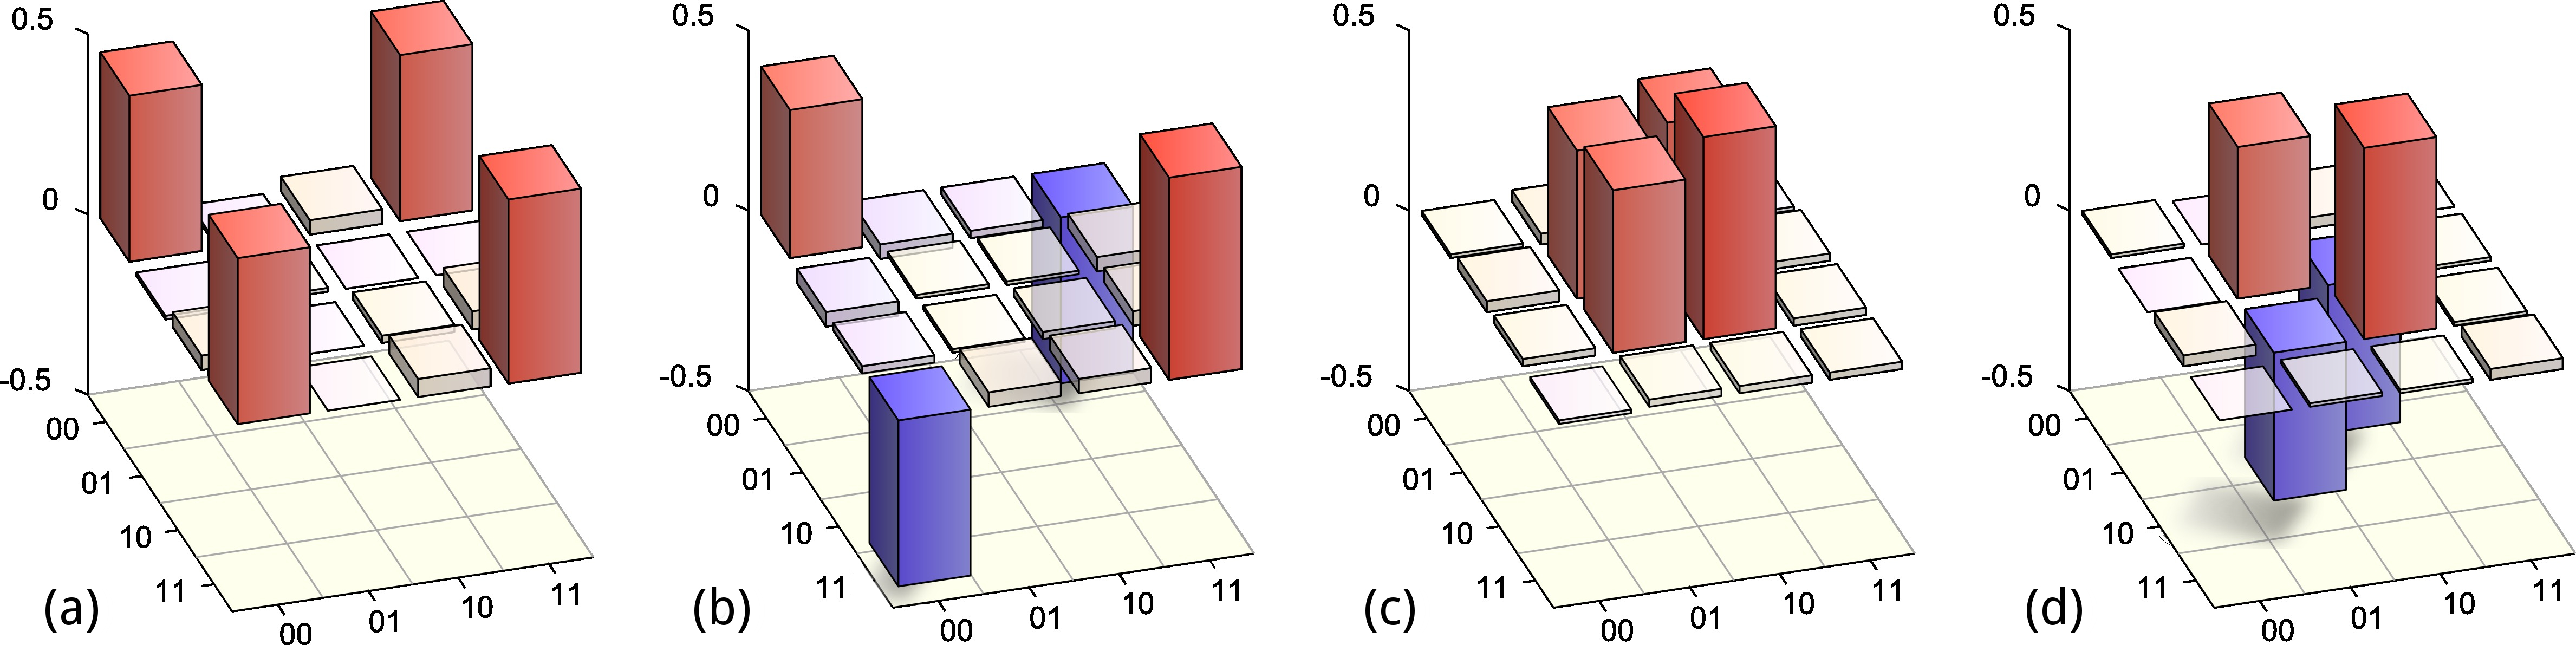
\includegraphics[width=1.0\linewidth]{chapter3/fig/4.jpg}
\caption[On-chip quantum state tomography]{
On-chip quantum state tomography.  
Density matrices of the Bell states (a) $\ket{\Phi^{+}}$, (b) $\ket{\Phi^{-}}$, (c) $\ket{\Psi^{+}}$ and (d) $\ket{\Psi^{-}}$,  generated and characterized on-chip. Imaginary parts are not shown. }
\label{fig:bells}
\end{figure}
% %%%%%%%%%%%%%%% End Bell state tomography figure

\subsection{On-chip quantum state tomography}
\label{sec:cnot-mz-tomography-experiment}
Throughout this thesis, we make use of \gls{qst} to characterize the quality of states generated by the \gls{cnotmz}. As a first demonstration, we prepared and measured each of the four canonical Bell states (\ref{eqn:bell-states}). These states, being maximally entangled, provide a particularly rigorous test of the performance of the \gls{cnotp} gate.

Setting appropriate voltages to phaseshifters $\phi_{1-4}$ as described in section \ref{sec:cnotmz-state-preparation}, we prepared the separable superposition states
\begin{equation}
   \ket{+}_C\otimes\ket{0}_T,\quad\ket{+}_C\otimes\ket{1}_T,\quad\ket{-}_C\otimes\ket{0}_T,\quad\ket{-}_C\otimes\ket{1}_T
\end{equation}
at the input of the \gls{cnotp} gate.  The corresponding Bell states ($\ket{\Phi^{\pm}}$ and  $\ket{\Psi^{\pm}}$ respectively) are then ideally produced at the output.

For each input state, phase shifters $\phi_{5-8}$ were then used to implement the quorum of 16 measurement settings required to reconstruct the density operator of the state. Since we collect statistics for all four logical outputs of the device simultaneously, is is straightforward to implement an over-complete quorum 
\begin{equation}
    \tmeas_i = \ket{C_i}\bra{C_i} \otimes \ket{T_i}\bra{T_i}
\end{equation}
over all combinations of $\ket{C_i}, \ket{T_i} \in \{\ket{0}, \ket{1}, \ket{+}, \ket{-}, \ket{+i}, \ket{-i}\}$.  
The measured density matrices of all four Bell states are shown in Fig. \ref{fig:bells}, with \emph{quantum state fidelities} \cite{Nielsen2004}
\begin{equation}
F=\left (Tr \sqrt{\sqrt{\rho_{th}} \rho_{exp} \sqrt{\rho_{th}} } \right)^{2} 
\label{eqn:quantum-state-fidelity}
\end{equation}
of  $0.947\pm0.002$, $0.945\pm0.002$, $0.933\pm0.002$, and $0.885\pm0.002$ respectively. 

A discussion of sources of error in the \gls{cnotmz}, to which we attribute the infidelity seen here, is given in section \ref{sec:cnotmz-discussion}.
%Since these measurements were first performed, the calibration procedure has been significantly improved and typical two-qubit quantum state fidelities are now closer to \SI{96}{\percent}.

\section{Quantum process tomography}
\label{sec:cnot-process-tomography}
\newcommand{\process}{\mathcal{E}}

\gls{qst} allows us to obtain complete information about the \emph{output} of a black-box source of quantum states. Often, we are also interested in devices which transform an arbitrary input state, where we would like to learn the \emph{a priori} unknown relationship between input and output states of the device \cite{White2007}.

While many of the errors which arise in \gls{loqc} are described by unitary operators\footnote{For example, errors in \gls{bs} reflectivity.}, in order to completely describe an arbitrary black-box device it is necessary to account for processes which do not preserve the purity or orthogonality of their input states. This can occur if the system couples to unknown environmental degrees of freedom, which are traced over in the final measurement. Any black box of this type can be completely and uniquely characterised by a completely positive map  $\process$. This operator describes the effect of the device on an input state $\dema_{in}$,
\begin{equation}
    \dema_{out} = \process\left( \dema_{in} \right) = \sum_i \hat{A}_i \dema_{in} \hat{A}_i^{\dagger}
\end{equation}
where $\hat{A}_i$ are a set of operators acting on the Hilbert space of $\dema$. In order to connect this theoretical description with experiment it is helpful to re-write 
\begin{equation}
    \hat{A}_i = \sum_j a_{i,j} \bar{A}_j
\end{equation}
where $\bar{A}_j$ are the Kraus operators, which are fixed and independent of $\process$. $\bar{A}_j$ satisfy $Tr (\bar{A}^{\dagger}_j \bar{A}_k ) \sim \delta_{j,k}$ and $\sum_j\bar{A}_j^{\dagger}\bar{A}_j = I$. For qubit systems the Kraus operators are typically chosen as tensor products of Pauli matrices, $\bar{A}_j = \hat{\sigma}_{j_0} \otimes \hat{\sigma}_{j_1} \otimes \ldots \otimes \hat{\sigma}_{j_n}$.
The quantum operation can then be completely and uniquely characterised by the \emph{process matrix} $\chi_{m,n} \equiv \sum_i{a_{i,m} a_{i,n}^{*}}$, a matrix of $2^{2n}$ complex numbers with $2^{4n}-2^{2n}$ free parameters, 
which relates $\dema_{out}$ to $\dema_{in}$ as 
\begin{equation}
    \dema_{out} = \process\left(\dema_\lin \right) = \sum_{m,n} \chi_{m,n} \bar{A}_{m} \dema_{in} \bar{A}_{n}^{\dagger}.
\end{equation}
The task of \gls{qpt} is then to estimate $\chi$. 
For an input state $\dema_\lin$, the probability that the output state of the device is detected in a state $\hat{\tau}_k$ is given by
\begin{equation}
    P_{jk} = 
    \mathrm{Tr} 
    \left[ \hat{\tau}_k \, \dema_\lout^j \right]  = 
    \mathrm{Tr} 
    \left[ \hat{\tau}_k \, \process \left( \dema_\lin^j \right) \right] .
\end{equation}
In order to obtain sufficient information to fully reconstruct $\process$ for an arbitrary device, we follow a procedure which is equivalent to full \gls{qst} of $\dema_\lout^j$, for a complete or over-complete set of linearly independent $\dema_\lin^j$ --- that is, $\dema_\lin^j$ should at least form a basis for the Hilbert space upon which $\process$ acts. 
Experimentally, we measure count rates 
\begin{equation}
    n_{jk} \approx P_{jk} \sum_j n_j = P_{jk} \mathcal{N}~;
    \quad
    \tilde{P}_{jk} \equiv \frac{n_{jk}}{\mathcal{N}}
\end{equation}
for every possible combination over a quorum of at least $4^n-1$ input states $\dema_\lin^j$ and $4^n-1$ measurement settings $\hat{\tau}_k$. 

Having acquired this data, we must then reconstruct $\chi$.
Although linear reconstruction techniques exist, they suffer the same issues as linear \gls{qst}: namely, experimental imperfection and finite statistics can lead to a reconstructed process matrix which is unphysical, precluding comparison with standard metrics.  
As a result, experimental \gls{qpt} is usually performed using a maximum-likelihood reconstruction technique.
As with maximum-likelihood \gls{qst}, we first choose a parametrization of $\chi$ which enforces physicality. 
Since the process matrix is subject to the same physical constraints as a density matrix (both are normalized, Hermitian, positive-semidefinite square matrices), we use a similar parametrization:
\begin{equation}
    \process(\vec{t}) \leftrightarrow \tilde{\chi}\left( \vec{t} \right) = 
    \frac{\hat{g}\left(\vec{t}\right) \hat{g}\left(\vec{t}\right)^{\dagger}}
    {\mathrm{Tr} \left[ \hat{g}\left(\vec{t}\right) \hat{g}\left(\vec{t}\right)^{\dagger} \right]}.
\end{equation}
We then minimize the cost function \cite{White2007}, constituting a least-squares difference between the observed data and that predicted by theory, with respect to $\vec{t}$:
\begin{equation}
    \Gamma(\vec{t}) = \sum_{jk} 
    \frac{
    \left(\tilde{P}_{jk} - 
    \mathrm{Tr} 
    \left[ \hat{\tau}_k \, \process (\vec{t} \dema_\lin^j) \right]
    \right)^2} {
    2 \mathrm{Tr} 
    \left[ \hat{\tau}_k \, \process (\vec{t} \dema_\lin^j) \right]
    }.
\end{equation}
Fortunately, this problem can be converted into a semidefinite program \cite{Ballo2010, LangfordThesis}, allowing the used of convex optimization algorithms which can greatly accelerate the numerical optimization procedure.

%%%%%%%%%%%%%% Begin quantum process tomography figure %%%%%%%%%%%%%%%
\begin{figure}[t!]
\centering
\includegraphics[width=\linewidth]{chapter3/fig/qpt_full.pdf}
\caption[Quantum process tomography of a maximally entangling gate.]{Quantum process tomography of a maximally entangling gate. (a) Ideal and experimental output states of the \gls{cnotp} gate, for a complete set of linearly independent input states. (b) Ideal process matrix of the \acrshort{cnot} gate. The imaginary part is zero everywhere. (c) Real and (d) imaginary parts of the measured process matrix of the \gls{cnotp} device, after a local rotation to permit comparison with the canonical \gls{cnot} gate.
}
\label{fig:qpt}
\end{figure}
%%%%%%%%%%%%%% End quantum process tomography figure %%%%%%%%%%%%%%%


\subsection{On-chip quantum process tomography}
\label{sec:expt-process-tomo}
We used the state preparation and measurement stages of the \gls{cnotmz} to perform full \gls{qpt} of the \gls{cnotp} gate. This test completely and uniquely characterizes the \gls{cnotp} gate itself, providing full information on the quality of our implementation. In addition, the \gls{qpt} protocol places stringent demands on the performance of the reconfigurable components of the chip: even if the \gls{cnotp} were perfect, errors in state preparation and measurement would lead to recovery of a flawed process matrix. Moreover, \gls{qpt} of a 2-qubit gate requires 256 measurements, and is particularly demanding in terms of repeatability and stability of the experimental setup.

Setting appropriate voltages to phase shifters $\phi_{1-4}$ as described in section \ref{sec:cnotmz-state-preparation}, we prepared 16 separable, linearly independent input states 
\begin{equation}
\rho^j_\lin = \ket{\Psi_j}{\bra{\Psi_j}}~ ; \quad
\ket{\Psi_j}=\ket{C_j}\otimes \ket{T_j}~ ; \quad
\ket{\psi} \in \{\ket{0}, \ket{1}, \ket{+}, \ket{+i} \ket{-i} \}.
\end{equation}
For each $\rho^j_\lin$, the output state of the \acrshort{cnotp} gate was measured and reconstructed by \gls{qst} as before, using phase shifters $\phi_{5-8}$ to perform each of the 16 measurements. These density matrices are shown together with ideal states in figure \ref{fig:qpt}(a).

The process matrix $\chi$ was then reconstructed according to the maximum likelihood technique previously described.
The experimentally measured process matrix is shown together with the theoretical ideal matrix $\chi_\mathrm{ideal}$ in figures \ref{fig:qpt}(b-d). For clarity, the experimental matrix has been rotated through a local two-qubit unitary which maps \gls{cnotp} to \gls{cnot} (see section \ref{sec:ralph-cnot}). The \emph{process fidelity} \cite{Nielsen2004}
\begin{equation}
F_{P} = \trace(\chi_\text{ideal}\chi_\text{exp})
\end{equation}
between the reconstructed process and the ideal \gls{cnot} operation was found to be 
0.841$\pm$ 0.002. 
This is comparable with the process fidelity of 0.87 previously measured using an equivalent bulk-optical circuit \cite{OBrien2004}. 
The average fidelity \cite{Gilchrist2009}, defined as the state fidelity between actual and ideal output states averaged over all possible input states, is 0.873$\pm$0.001. 
Here error was determined by a Monte-Carlo approach, assuming Poissonian photon statistics. 
Sources of error contributing to this sub-unit process fidelity are discussed in section \ref{sec:cnotmz-discussion}.

\begin{figure}[t!]
\centering
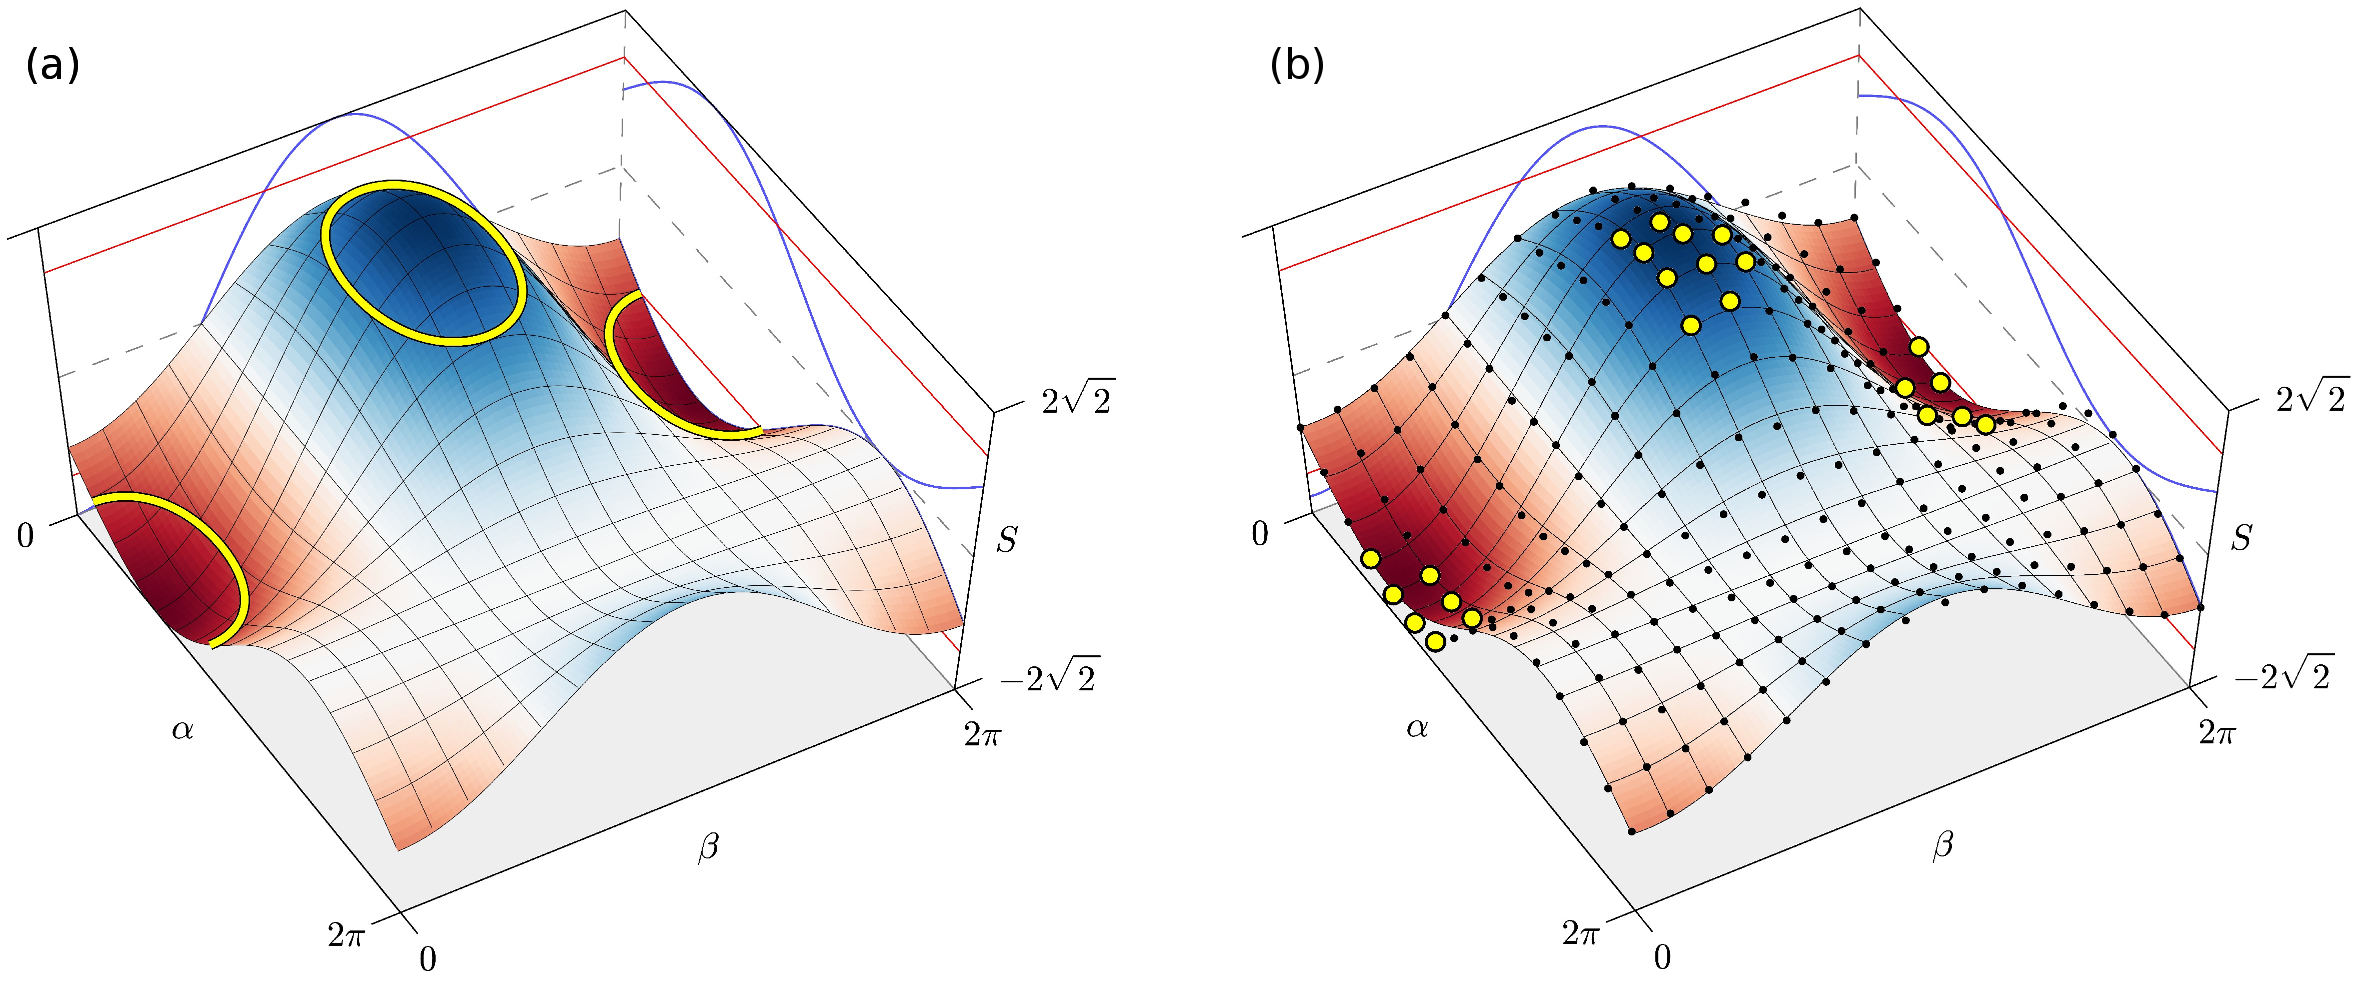
\includegraphics[width=.9\linewidth]{chapter3/fig/5.jpg}
\caption[CHSH manifold.]{\acrshort{chsh} manifold.
(a) The Bell-\acrshort{chsh} sum $S$, plotted as a function of phases $\alpha$ and $\beta$. In the $\alpha$ axis, the state shared between Alice and Bob is tuned continuously between product states at $\alpha=0, \pi$ and maximally entangled states at $\alpha=\pi/2, 3\pi/2$. The $\beta$ axis shows $S$ as a function of Bob's variable measurements, which can be thought of as two operator-axes in the real plane of the Bloch sphere, fixed with respect to each other at an angle of $\pi/2$ but otherwise free to rotate with angle $\beta$ between 0 and $2\pi$. The blue curves show a projection of the manifold onto each axis. Yellow contours mark the edges of regions of the manifold which violate $-2 \le S\le 2$. Red lines on the axes also show this limit.
(b) Experimentally measured manifold. Data points are drawn as black circles. Data points which violate the \acrshort{chsh} inequality are drawn as yellow circles. The surface shows a fit to the experimental data.}
\label{fig:chsh}
\end{figure}

\section{Bell inequality manifold}
\label{sec:cnot-mz-chsh}
Having shown that the \gls{cnotmz} can prepare maximally entangled states, we now demonstrate that these states are nonlocal.
As previously discussed, the Bell-\gls{chsh} test (section \ref{sec:nonlocality}) provides a particularly rigorous criterion for a source of entanglement. In particular, only a subset of the most strongly entangled states can generate nonlocal statistics in a \gls{chsh} test. As such, \gls{chsh} is important not only as a fundamental test of foundational quantum theory, but also as a measure of the operational performance of quantum technologies and devices.

In the context of the \gls{cnotmz}, all local realistic models demand that 
\begin{equation}
    |S|=|\expect{\hat{C_1}\hat{T_1}}
        +\expect{\hat{C_1}\hat{T_2}}
        +\expect{\hat{C_2}\hat{T_1}}
        -\expect{\hat{C_2}\hat{T_2}}| \le 2
        \label{eqn:cnotmz-chsh}
\end{equation}
where $\hat{C}_i$, $\hat{T}_j$ are measurement operators on the control and target qubits respectively.  If these qubits are entangled, this inequality can be violated up to a maximum value of $|S|=2\sqrt{2}$ --- in which case we say that we detect nonlocal statistics, or that we ``obtain nonlocality''. 


In order to further test the reconfigurability of the \gls{cnotmz}, we measured $S$ over a range of partially entangled states, using a variety of measurement settings.
%Nonlocality is only obtained when the two-qubit state $\ket{\Psi (\phi_{1-4})}$ generated by the \gls{cnotp} gate is sufficiently entangled. 
%Moreover, 
Even if the state $\ket{\Psi (\phi_{1-4})}$ generated by the \gls{cnotp} is maximally entangled, (\ref{eqn:cnotmz-chsh}) is only violated for a subset of measurement settings. See section \ref{sec:random-chsh-calibrated} for further discussion of this point.

We used $\phi_{1-4}$, together with the \acrshort{cnotp} gate, to prepare the state
\begin{equation}
\ket{\psi_{out}}=\frac{1}{2\sqrt{2}} \left [ \left ( 1-e^{i\alpha} \right ) \ket{00} + \left(1+e^{i\alpha} \right)\ket{11} \right ],
\end{equation}
where $\alpha=\phi_{1}$ tunes continuously between two orthogonal states: for $\alpha=0,\pi$, $\ket{\psi_{out}}$ is a product state, and with $\alpha=\pi/2,3\pi/2$, $\ket{\psi_{out}}$ is the maximally entangled state $\frac{1}{\sqrt{2}} \left ( \ket{00} \pm i \ket{11} \right )$ (up to a global phase). Scanning $\alpha$ in the interval $\left[0, 2\pi\right]$, we pass through a continuum of partially entangled states.
In order to evaluate $S$, we used phaseshifters $\phi_{5-8}$ to implement four two-qubit measurements on the state emerging from the \acrshort{cnotp} gate. 
%%%%
While Alice's measurement settings ($\phi_6 \in \{ \pi / 4, -\pi/4 \}$) were fixed, 
Bob's measurement operators were continuously rotated in the real plane of the Bloch sphere, with $\phi_8 \in \{\beta, \beta+\pi/2\}$. 
%%%%
We measured $S(\alpha, \beta)$ for $\alpha \in [0,2\pi]$ and $\beta \in [0, 2\pi]$, with step size $2\pi/15$, producing the ``Bell manifold'' shown in figure \ref{fig:chsh}. We measured maximum and minimum values of $S$ of $2.49\pm0.03$ and $-2.54\pm0.03$ respectively. Errors were again determined by a Monte-Carlo technique, assuming Poissonian statistics. 

In order to quantitatively compare the theoretical manifold with experimental data, we used the quantity \begin{equation}R^{2}=1-\frac{\sum_{i} (S_{i}-T_{i})^{2}}{\sum_{i} (S_{i}-\bar{S})^{2}},\end{equation} where $S_{i}$ are experimentally measured values of the Bell-\acrshort{chsh} sum, $\bar{S}$ is the average over $S_{i}$, and $T_{i}$ are the theoretical values of $S$ shown in Fig. \ref{fig:chsh}a. In the ideal case, $R^2=1$. For the data shown in figure \ref{fig:chsh}b, $R^2=0.935$.

\section{Generating and characterising mixture}
\label{sec:cnotmz-mixture}

Mixture, introduced in section \ref{sec:background-mixture}, is a basic property of quantum mechanical states, equivalent to classical randomness. The effect of decoherence, which is the major source of errors in many proposed architectures for quantum computing, is to introduce mixture to the computer's state, and the study and modelling of mixed states will be important in future studies of decoherence mechanisms.  Despite this broad association of mixture with error, mixed states can actually be used for universal quantum computing \cite{Lanyon2008a}, and are believed to play an important role in biological processes \cite{Mohseni2008a, Plenio2008a} including photosynthesis. 

One approach to generating mixed states is to build a source which randomly samples from an ensemble of pure states: for example, to generate the maximally-mixed single-qubit state $\identity/2$, we can use a source which generates each of the logical basis states with equal probability
\begin{equation}
    \dema = \sum_i p_i \ket{i} \bra{i} 
    = \frac{1}{2}\ket{0} \bra{0} + \frac{1}{2}\ket{1}\bra{1} 
    = \identity/2.
\end{equation}
Note that in this approach, it is important that the random sampling technique, which chooses between $\ket{0}$ and $\ket{1}$, must not ``leak'' information to the observer --- otherwise the state can be written in a pure form:
\begin{equation}
    \ket{0_{t_1} 1_{t_2} 1_{t_3} 0_{t_4} 0_{t_5} 1_{t_6} \ldots}
\end{equation}
An alternative approach\footnote{Note: these two forms of mixture are sometimes distinguished as \emph{improper} (using entangled states) and \emph{proper} (using a random number generator). However, they are formally indistinguishable \cite{Masillo2009}.} begins with a maximally entangled, pure, two-qubit state, and traces over one qubit:
\begin{equation}
    \dema_A = \mathrm{Tr}_B\left[
        \frac{1}{\sqrt{2}}\left(
        \ket{0_A0_B}+
        \ket{1_A1_B}
    \right)
    \right]
    = \frac{1}{2}\ket{0} \bra{0} + \frac{1}{2}\ket{1}\bra{1} 
    = \identity/2.
\end{equation}
The \gls{cnotmz} can prepare an arbitrary two-qubit state (section \ref{sec:arbitrary-two-qubit}), and by tracing over one qubit can thus prepare arbitrary single-qubit mixed states. Starting from the parametrization (\ref{eqn:schmidt-state}) of an arbitrary two qubit state, and tracing over the target qubit
\begin{align}
  \ket{\Psi_{CT}} 
  &= \sqrt{\lambda} \, \ket{\lambda_C} \otimes \ket{\lambda_T }
  + \sqrt{1-\lambda} \, \ket{\lambda_C ^ \perp} \otimes \ket{\lambda_T ^ \perp}\\
  \xrightarrow{\mathrm{trace}}
   \dema_C 
   &= \mathrm{Tr}_T \left(
      \ket{\Psi}\bra{\Psi}
  \right)
  = \lambda \ket{\lambda_C}\bra{\lambda_C} +
  (1-\lambda) \ket{\lambda_C^\perp}\bra{\lambda_C^\perp}
  \label{eqn:mixed-output}
\end{align}
Since $\ket{\lambda_C}$ is an arbitrary single-qubit pure state, $\dema_C$ is an arbitrary mixed state. Note that there is a one-to-one correspondence between the degree of entanglement of the initial two-qubit state and the purity of the reduced density matrix, dictated by the choice of $\lambda$.

What does it mean to ``trace over the target qubit'' in the context of the \gls{cnotmz}? Ideally, we would measure the control qubit independent of the target qubit, which in principle need not be measured at all. However, since the \gls{cnotp} is a nondeterministic gate, we must count in the coincidence basis to postselect on successful gate operation. Therefore, in practice we count coincidences across both qubits and then combine two-photon count-rates to generate effective single-qubit data, independent of the measurement outcome on the target:
\begin{equation}
    \tilde{c}_{0_C} = c_{0_C0_T} + c_{0_C1_T} ~; \quad 
    \tilde{c}_{1_C} = c_{1_C0_T} + c_{1_C1_T}.
\end{equation}

\begin{figure}[t!]
\centering
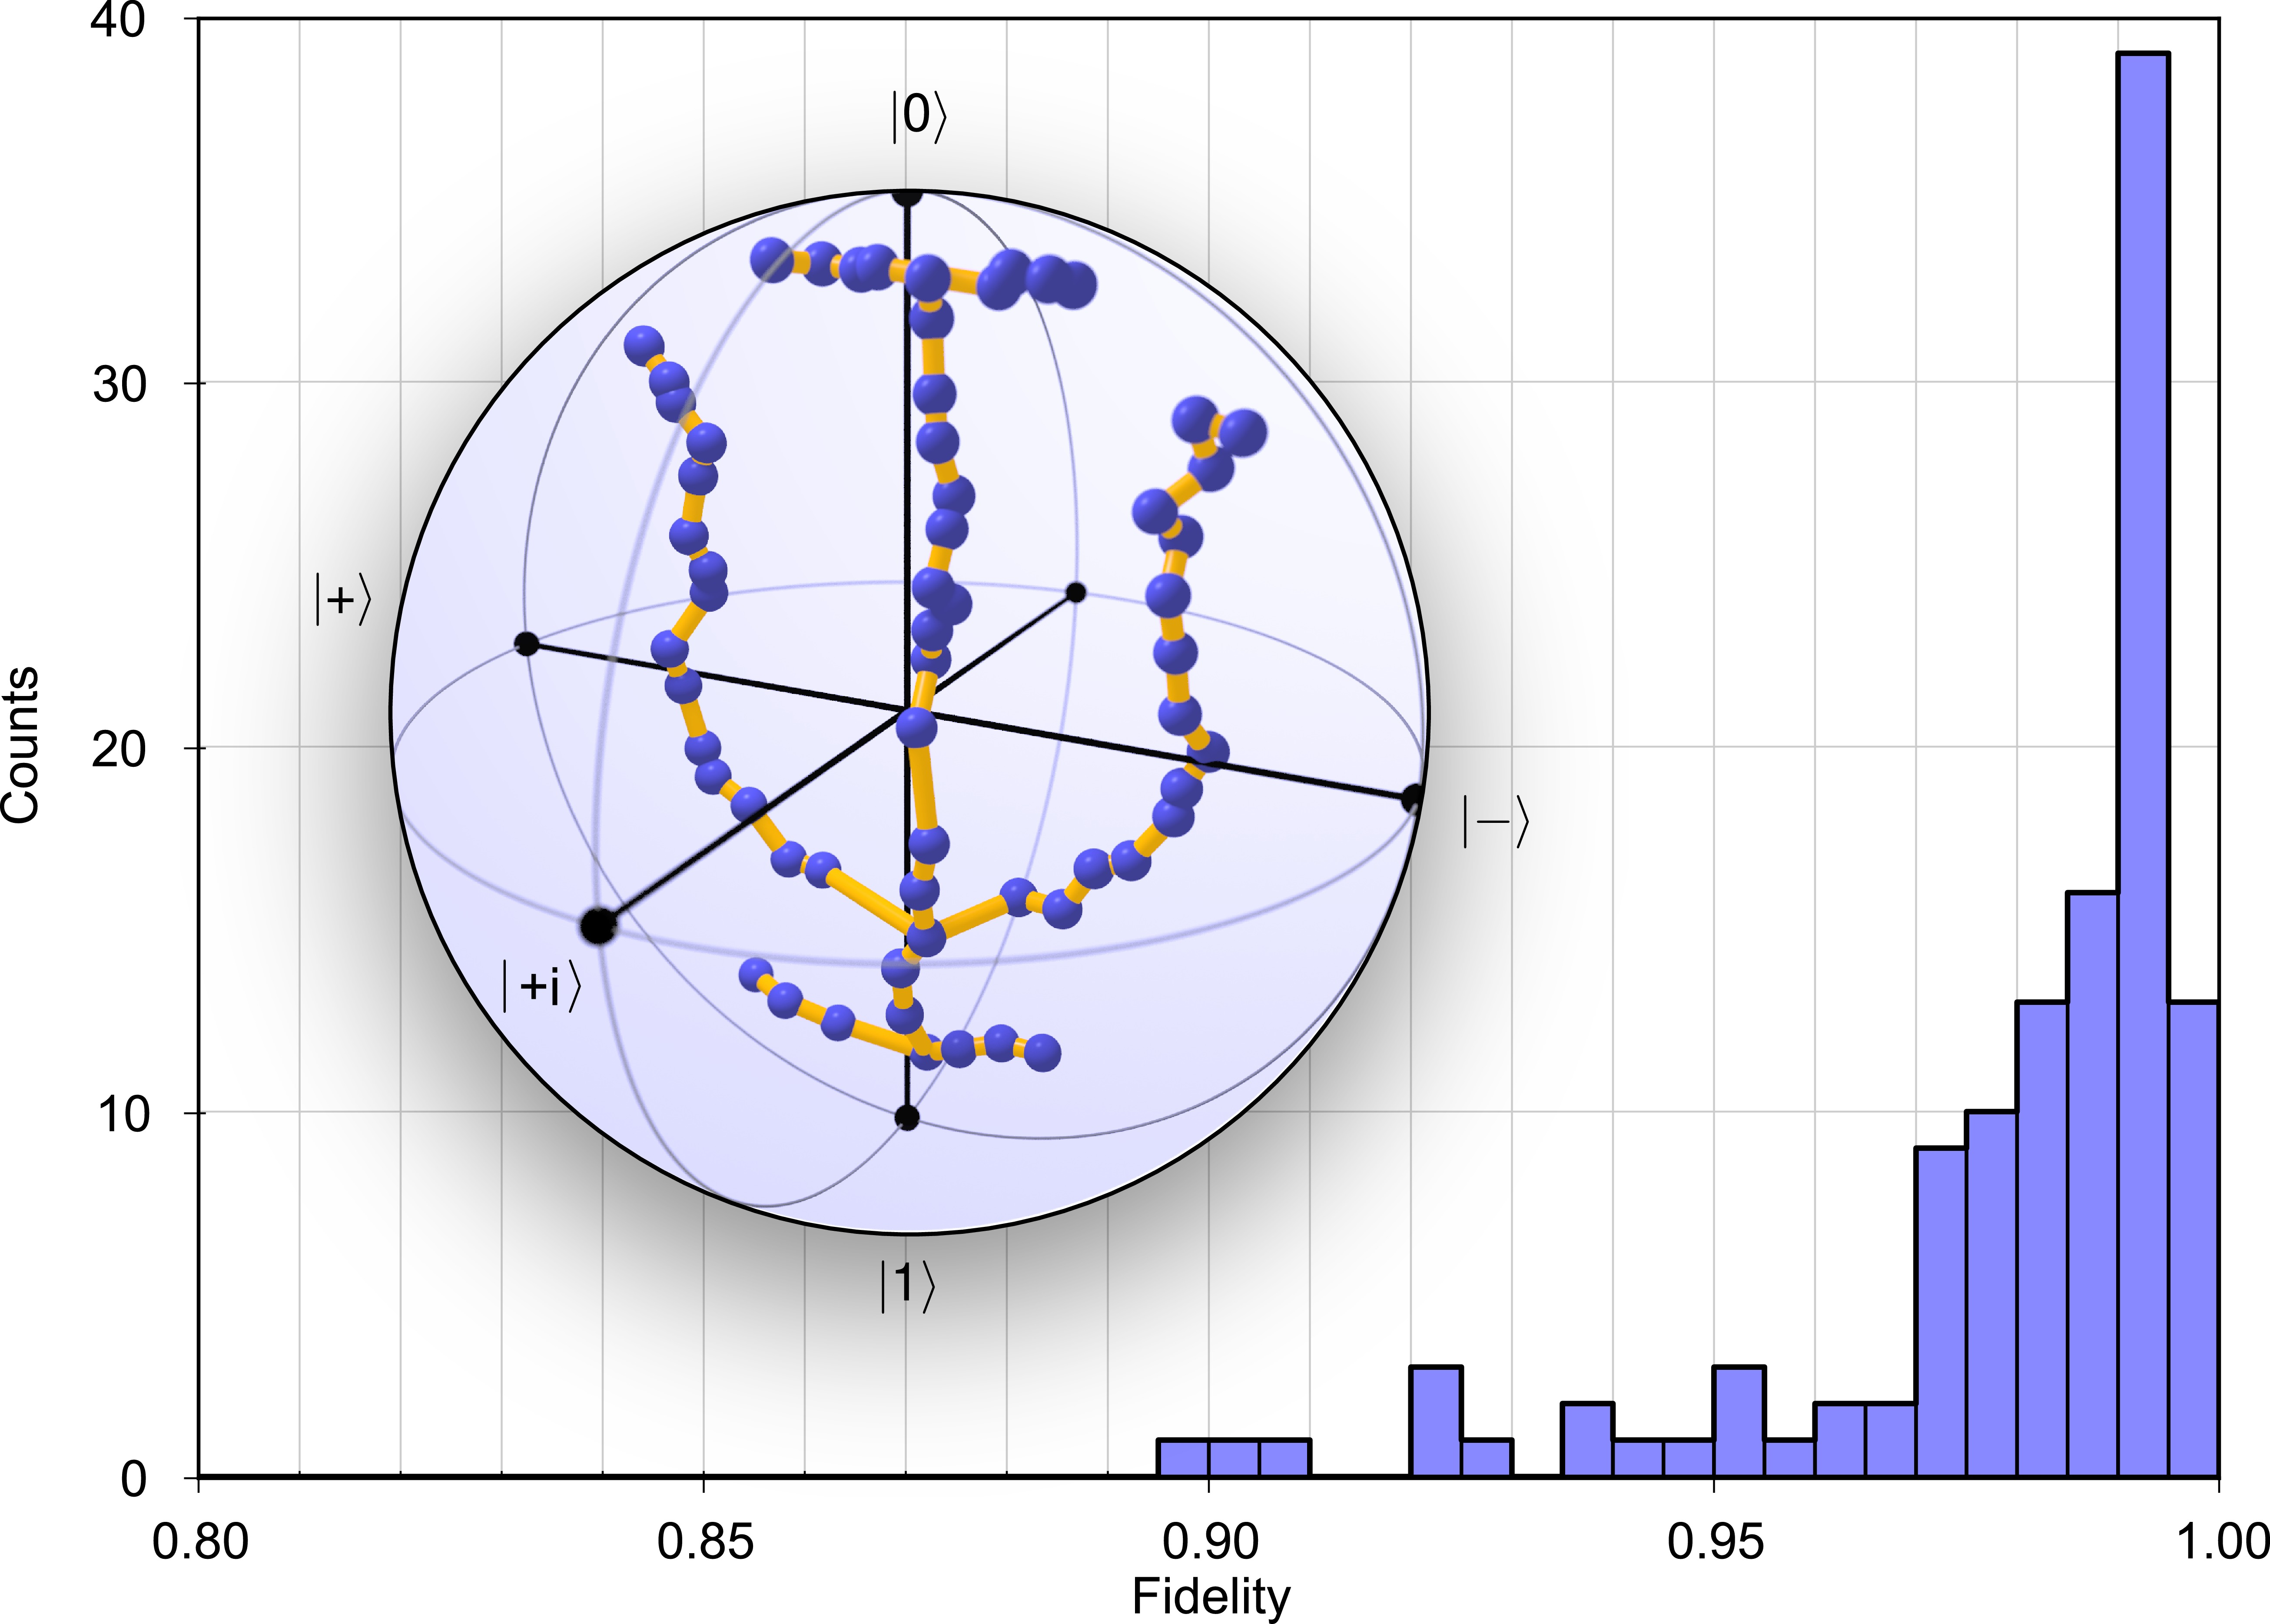
\includegraphics[width=.8\linewidth]{chapter3/fig/6.jpg}
\caption[Generating mixed states]{Histogram showing the statistical distribution of quantum state fidelity between 119 randomly chosen single-qubit target states and the corresponding mixed states generated and characterized on-chip. Inset: $\Psi$ drawn in the Bloch sphere using 63 mixed states, again generated and characterized on-chip. These states are chosen from the real plane of the sphere for clarity. The point at the centre of the sphere is maximally mixed, and was traced out from a two-qubit maximally entangled state. Points on the surface of the sphere are pure, and were traced out from separable states.}
\label{fig:mixedstates}
\end{figure}


We chose 119 single-qubit mixed states of varying purity, at random by the Hilbert-Schmidt measure \cite{Zyczkowski2001}, which samples uniformly from the full volume of the Bloch sphere.
For each mixed state, we generated an appropriate two-qubit pure state, traced out the target qubit, and performed full single-qubit \gls{qst} on the control, reconstructing the reduced density matrix based on $\tilde{c}_{0_C}$, $\tilde{c}_{1_C}$.
Figure \ref{fig:mixedstates} shows the distribution of quantum state fidelity (\ref{eqn:quantum-state-fidelity}) between reconstructed states and their corresponding ideal mixed states. The average fidelity across all 119 states was found to be $0.98\pm0.02$, with 91\% of states having fidelity $> 0.95 $. We then chose 63 specific mixed states that mapped out the symbol `$\Psi$' inside the Bloch sphere, and generated them with high fidelity (figure \ref{fig:mixedstates}, inset). This picture gives a visual impression of the typical fidelity with which mixed states (and, by implication, entangled states) can be prepared and measured using the \gls{cnotmz}.


\subsection{Errors in the \acrshort{cnotmz}}
\label{sec:cnot-mz-errors}
\begin{figure}[t!]
\centering
\includegraphics[width=.8\linewidth]{chapter3/fig/errors.pdf}
\caption[Errors in the \acrshort{cnotmz}]
{Errors in the \gls{cnotmz}. Solid lines show a numerical simulation, plotting quantum state fidelity of states reconstructed by maximum-likelihood \gls{qst} against the visibility of \gls{hom} interference. The grey line assumes perfect phaseshifters and infinite statistics, while the black line models the effect of \SI{0.05}{\radian} variance in phase on each phaseshifter, as well as the effects of finite statistics for a realistic experimental count-rate. The red line shows the experimentally measured visibility of \gls{hom} interference, and red crosses show measured quantum state fidelities of the four Bell states.}
\label{fig:cnotmz-errors}
\end{figure}

The imperfect performance of the \gls{cnotmz} seen in the previous experiments can be attributed to a number of different sources of error. First, we do not achieve perfect \gls{hom} interference, due to residual distinguishability of the photon pair --- this is likely due to small polarization rotations, temporal distinguishability, and imperfect mode-matching at the \glspl{dc}. A larger fraction of error is due to imperfect calibration and operation of the thermal phaseshifters, which contributes significantly to imperfection in reconstructed states and processes. Figure \ref{fig:cnotmz-errors} shows the effect of inaccuracy in the control of phases in the \gls{cnotmz}: the fidelity of states reconstructed by \gls{qst} is reduced by \SI{\sim 4}{\percent} given \SI{0.05}{\radian} of variance at each phaseshifter. We expect that imperfect fabrication of passive waveguide structures in the \gls{cnotmz}, which leads to time-invariant unitary errors and is reflected in the results of section \ref{sec:expt-process-tomo}, accounts for the remaining discrepancy between our experiment and the ideal performance of the device.

\section{Discussion}
\label{sec:cnotmz-discussion}
In this chapter, we have not shown any new ability to manipulate quantum states which could not be duplicated in practice using bulk optics.
The \acrshort{cnotp} gate \cite{OBrien2003}, experimental state and process tomography \cite{OBrien2004}, and mixed-state preparation have all previously been shown in bulk. 
The main result of work presented in this chapter is instead to show that the complexity and flexibility of bulk optics for quantum information can be reproduced to equivalent or better fidelity in a waveguide chip. This represents a significant step forward with respect to previous experiments in integrated quantum photonics, where devices were either completely passive \cite{Politi2009, Politi2009a, Peruzzo2011a, Marshall2009, Matthews2011a}
or insufficiently complex/reconfigurable to perform multiple distinct tasks
\cite{Matthews2009, Politi2009}.  

A side-effect of photonic integration is the ease with which the circuit can be fully automated, enabling experiments which depend on a large number of measurements (chapters \ref{chap:delayed-choice} and \ref{chap:random-chsh}), or feedback and optimization over a large number of experimental parameters (chapter \ref{chap:quantum-chemistry}). Automation to this extent can be experimentally demanding or expensive  in bulk-optics.

There remains considerable scope for improvement of the experimental setup and device fabrication. First, the silica-on-silicon material system used here is intrinsically limited by the available refractive index contrast, which leads to relatively large devices. A competitive quantum information processor built in silica-on-silicon would likely be prohibitively large. Recently, there has been great progress in integrated quantum optics using material systems which allow for a much higher component density: in particular, silicon nanowire waveguides \cite{Silverstone2013, Matsuda2012, Azzini2012, Takesue2008, Sharping2006, Bonneau2012, Martin2012}, can provide up to six orders of magnitude decrease in component size. 

As discussed in section \ref{sec:cnot-mz-errors}, inaccuracy in phaseshifter calibration is significantly detrimental to the performance of the device. Recently, Li et al. \cite{Li2013} have shown a new method for calibration of the \gls{cnotmz}, using a Bayesian learning method to automatically find the optimal calibration settings. The authors report significant improvements in the performance of the device, with respect to those reported here.

%FUTURE: sources and detectors on chip

To summarize, we have shown an integrated quantum photonic chip with a considerably greater degree of reconfigurability than previous devices. We have demonstrated the ability of this chip to generate arbitrary two-qubit entangled states and single-qubit mixed states. We have confirmed the entangling capability of the device through violation of a Bell inequality across a large fraction of the parameter space. Finally, we have completely characterised the quantum process implemented by the \gls{cnotp} gate by \gls{qpt}. To our knowledge, in the field of integrated quantum photonics, this work constitutes the first demonstration of quantum state and process tomography where state preparation and measurement were both implemented on-chip, as well as the first on-chip Bell violation.  
The general-purpose utility of the \gls{cnotmz} is borne out in the following chapters.

\section*{Statement of work}
I optimized the photon source, and found and optimized the Hong-Ou-Mandel dip. I built, optimized and programmed a large fraction of the supporting electronics. I calibrated the resistive heaters, and designed and optimized the pulse sequence described in section \ref{sec:control-automation-readout}. I measured all of the experimental data, and performed all of the simulations shown in this section. I conceived the randomized characterization protocol.

% References
\bibliographystyle{unsrt}
\bibliography{main.bib}
